\section{问题一：主流大语言模型综合性能评价}

\subsection{问题分析}

大语言模型的综合性能具有明显的多维特征。不同模型在复杂推理、知识与事实可靠性、长上下文处理、代码与软件工程以及多模态任务上的表现存在差异，仅依赖单一 Benchmark 难以全面反映模型的能力结构。

本题数据具有三个特点。第一，不同 Benchmark 的评分尺度、测试难度和评价协议并不统一，原始得分不具有直接可加性。第二，不同 Benchmark 之间可能存在信息重叠，若将高度相关的指标重复计入综合评价，可能造成隐性重复赋权。第三，各模型公开测评结果并不完整，部分指标存在由模型功能差异造成的结构性缺失。例如，多模态指标仅适用于具备相应能力且存在公开结果的模型，不能将未适用或未公开结果简单视为零分。

基于上述特点，本文不直接对原始 Benchmark 分数加权平均，而以模型在同一 Exact Setting 下的相对优劣关系为基本信息，构建基于成对比较的综合评价模型。模型路线为：Missing-aware Spearman 相关分析、Benchmark Family 筛选、Family-balanced Margin-weighted 成对比较、正则化 Bradley--Terry 模型、C1--C5 潜在能力估计、信息--冗余--稳定性客观赋权、缺失感知综合评分，以及 Bootstrap、Leave-One-Family-Out（LOFO）和敏感性分析。

问题一的总体建模框架见图~\ref{fig:q1_framework}。由图~\ref{fig:q1_framework}可知，本文先完成数据审计、缺失结构识别和五维指标体系构建，再在 Exact Setting 层形成可比的模型成对关系，最终通过客观赋权和稳健性检验得到综合排名及 Kimi K3 的能力结构判断。

\begin{figure}[htbp]
    \centering
    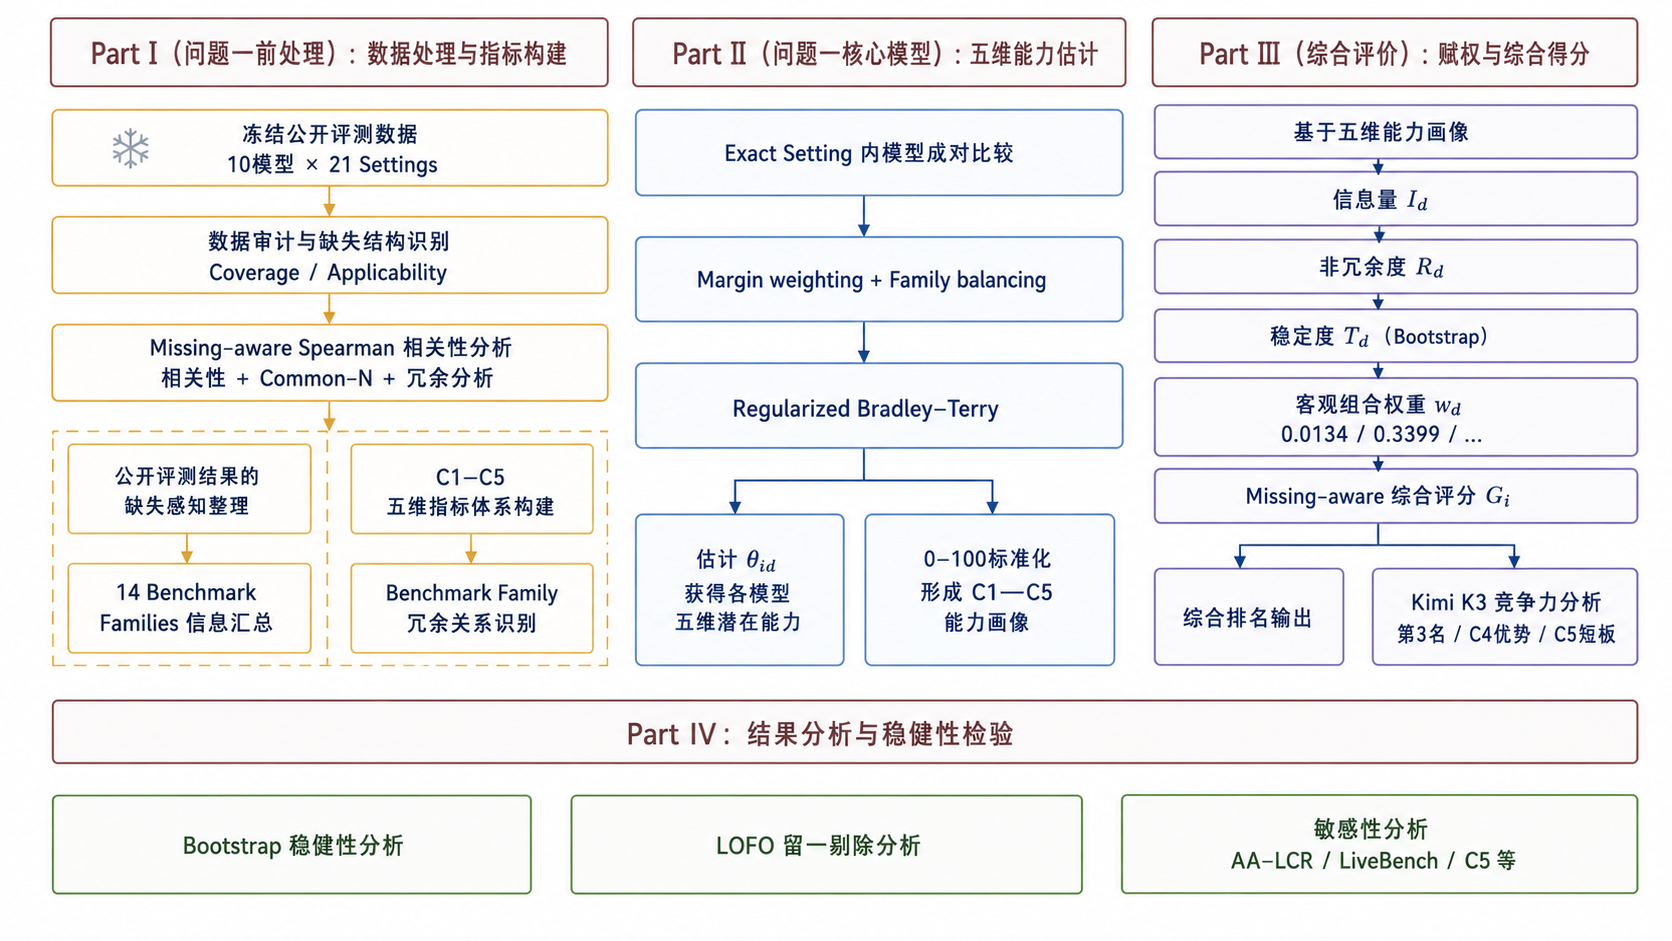
\includegraphics[width=\textwidth]{outputs/q1/figures/figure_q1_00_model_framework.png}
    \caption{问题一综合评价模型总体框架}
    \label{fig:q1_framework}
\end{figure}

\subsection{数据与指标体系}

\subsubsection{数据集构成}

本文以具体模型版本为评价对象，选取 10 个主流大语言模型，包括 Kimi K3 (max reasoning)、GPT-5.6 Sol (max)、GPT-5.5 (xhigh)、Claude Fable 5 (max, with fallback)、Claude Opus 4.8 (max)、Gemini-3.1-Pro (High)、DeepSeek-V4-Pro Max、DeepSeek-V4-Flash Max、Qwen3.8-Max 和 GLM-5.2 (max)。

经模型版本匹配、公开结果核验和人工复核后，正式冻结数据版本为 v1.0，冻结日期为 2026-08-17。该版本包含 14 个 Benchmark Families 和 21 个 Exact Settings，理论上形成 \(10\times21=210\) 个“模型--测试设置”组合，其中获得有效观测 164 项。整体数据覆盖率定义为
\begin{equation}
\eta
=
\frac{N_{\mathrm{obs}}}{N_{\mathrm{model}}N_{\mathrm{setting}}}
=
\frac{164}{10\times21}
=0.7810.
\label{eq:q1_coverage}
\end{equation}
式~\eqref{eq:q1_coverage} 表明，当前核心矩阵覆盖率为 \(78.10\%\)。全部 164 项核心记录均完成来源追溯与人工核验，SHA-256 校验通过。各模型的数据覆盖情况见表~\ref{tab:q1_model_coverage}。由表~\ref{tab:q1_model_coverage}可知，Kimi K3 的 Exact Setting 覆盖率为 \(85.71\%\)，最低单模型覆盖率为 \(66.67\%\)。

\begin{table}[htbp]
\centering
\caption{模型数据覆盖情况}
\label{tab:q1_model_coverage}
\begin{tabular}{lccc}
\toprule
模型 & 有效设置数 & 总设置数 & 覆盖率 \\
\midrule
Kimi K3 (max reasoning) & 18 & 21 & 0.857 \\
GPT-5.6 Sol (max) & 17 & 21 & 0.810 \\
GPT-5.5 (xhigh) & 17 & 21 & 0.810 \\
Claude Fable 5 (max, with fallback) & 17 & 21 & 0.810 \\
Claude Opus 4.8 (max) & 16 & 21 & 0.762 \\
Gemini-3.1-Pro (High) & 16 & 21 & 0.762 \\
DeepSeek-V4-Pro Max & 17 & 21 & 0.810 \\
DeepSeek-V4-Flash Max & 16 & 21 & 0.762 \\
Qwen3.8-Max & 14 & 21 & 0.667 \\
GLM-5.2 (max) & 16 & 21 & 0.762 \\
\bottomrule
\end{tabular}
\end{table}

模型--Exact Setting 覆盖结构见图~\ref{fig:q1_coverage_heatmap}。由图~\ref{fig:q1_coverage_heatmap}可知，数据缺失并非完全随机，C5 多模态维度只覆盖具有相应公开多模态测评结果的模型。因此，后续综合评价采用缺失感知处理，不对缺失单元进行插补。

\begin{figure}[htbp]
    \centering
    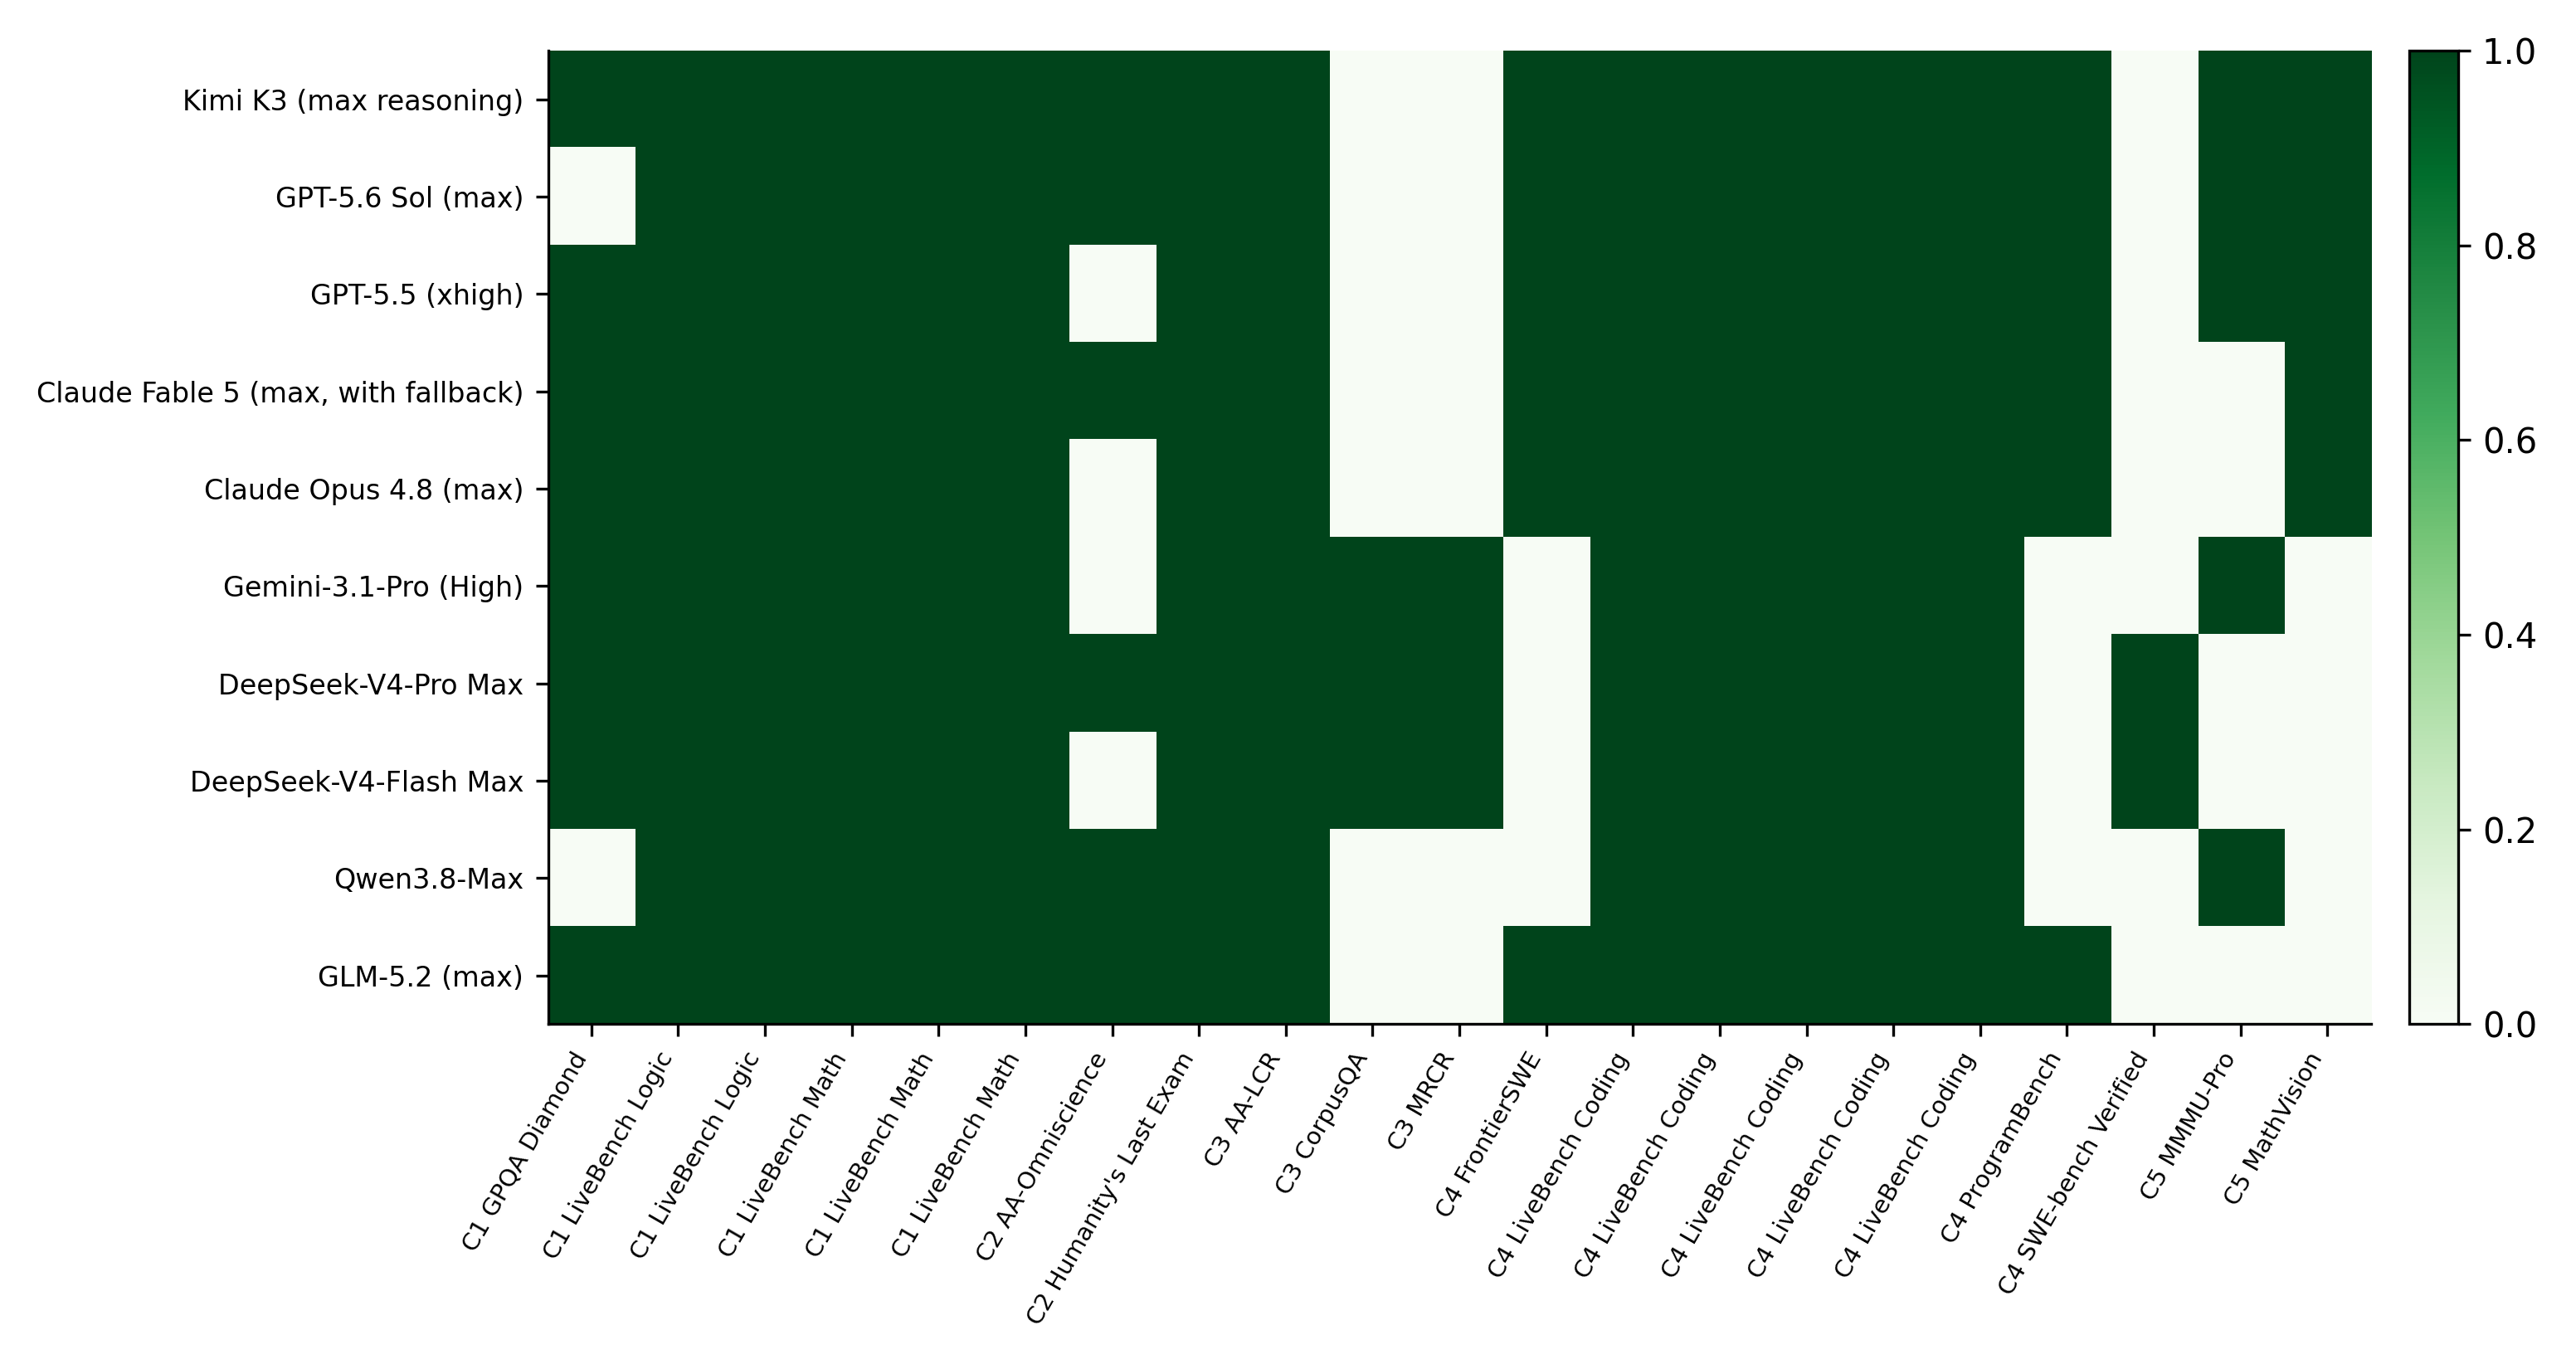
\includegraphics[width=0.92\textwidth]{outputs/q1/figures/figure_q1_01_coverage_heatmap.png}
    \caption{模型--Exact Setting 数据覆盖热力图}
    \label{fig:q1_coverage_heatmap}
\end{figure}

\subsubsection{分层指标体系}

考虑到同一能力可由多个 Benchmark Family 共同刻画，而同一 Benchmark Family 内又可能包含多个 Exact Settings，本文构建“综合性能--能力维度--Benchmark Family--Exact Setting”的四层评价结构。Exact Setting 是可直接进行模型间比较的最小单元；Benchmark Family 用于归并评价目标相同或高度接近的测试设置；能力维度用于反映模型的一级能力结构。

五个一级能力维度定义为：\(C_1\) 复杂推理、\(C_2\) 知识与事实可靠性、\(C_3\) 长上下文、\(C_4\) 代码与软件工程、\(C_5\) 多模态。指标体系见表~\ref{tab:q1_indicator_system}。

\begin{table}[htbp]
\centering
\caption{C1--C5 与 Benchmark Family 指标体系}
\label{tab:q1_indicator_system}
\resizebox{\textwidth}{!}{
\begin{tabular}{llccc}
\toprule
能力维度 & Benchmark Family & Exact Settings 数 & 主要度量 & 模型覆盖率 \\
\midrule
C1 复杂推理 & GPQA Diamond & 1 & Accuracy & 0.8 \\
C1 复杂推理 & LiveBench Logic & 2 & Task score & 1.0 \\
C1 复杂推理 & LiveBench Math & 3 & Task score & 1.0 \\
C2 知识与事实可靠性 & AA-Omniscience & 1 & Omniscience Index & 0.6 \\
C2 知识与事实可靠性 & Humanity's Last Exam & 1 & Accuracy & 1.0 \\
C3 长上下文 & AA-LCR & 1 & Accuracy & 1.0 \\
C3 长上下文 & CorpusQA & 1 & ACC & 0.3 \\
C3 长上下文 & MRCR & 1 & MMR & 0.3 \\
C4 代码与软件工程 & FrontierSWE & 1 & Dominance score & 0.6 \\
C4 代码与软件工程 & LiveBench Coding & 5 & Task score & 1.0 \\
C4 代码与软件工程 & ProgramBench & 1 & Accuracy & 0.6 \\
C4 代码与软件工程 & SWE-bench Verified & 1 & Resolved & 0.2 \\
C5 多模态 & MMMU-Pro & 1 & Accuracy & 0.5 \\
C5 多模态 & MathVision & 1 & Accuracy & 0.5 \\
\bottomrule
\end{tabular}}
\end{table}

\subsection{指标相关性和筛选}

由于不同 Benchmark 的有效模型集合并不完全一致，若先对缺失值进行插补再计算相关系数，会人为引入不存在的数据关系。因此，本文采用基于共同有效样本的 Spearman 秩相关系数。设 Benchmark \(j\) 与 Benchmark \(k\) 的共同有效模型集合为
\begin{equation}
I_{jk}
=
\{\,i\mid x_{ij}\ \text{与}\ x_{ik}\ \text{均存在}\,\},
\qquad
n_{jk}=|I_{jk}|.
\label{eq:q1_spearman}
\end{equation}
基于该集合，二者的缺失感知 Spearman 相关系数为
\begin{equation}
\rho_{jk}
=
\operatorname{Spearman}
\left(
X_j^{(I_{jk})},
X_k^{(I_{jk})}
\right).
\label{eq:q1_spearman_coef}
\end{equation}
式~\eqref{eq:q1_spearman} 同时保留共同样本数 \(n_{jk}\)，式~\eqref{eq:q1_spearman_coef} 给出相应秩相关系数。这是因为在缺失数据条件下，相关系数的解释不仅取决于系数大小，也取决于实际参与计算的模型数量。

Benchmark Family 的 Spearman 相关热力图见图~\ref{fig:q1_spearman_heatmap}。由图~\ref{fig:q1_spearman_heatmap}可知，部分 Benchmark Family 之间存在较高相关性，例如 AA-Omniscience 与 Humanity's Last Exam、MMMU-Pro 与 MathVision 等。

\begin{figure}[htbp]
    \centering
    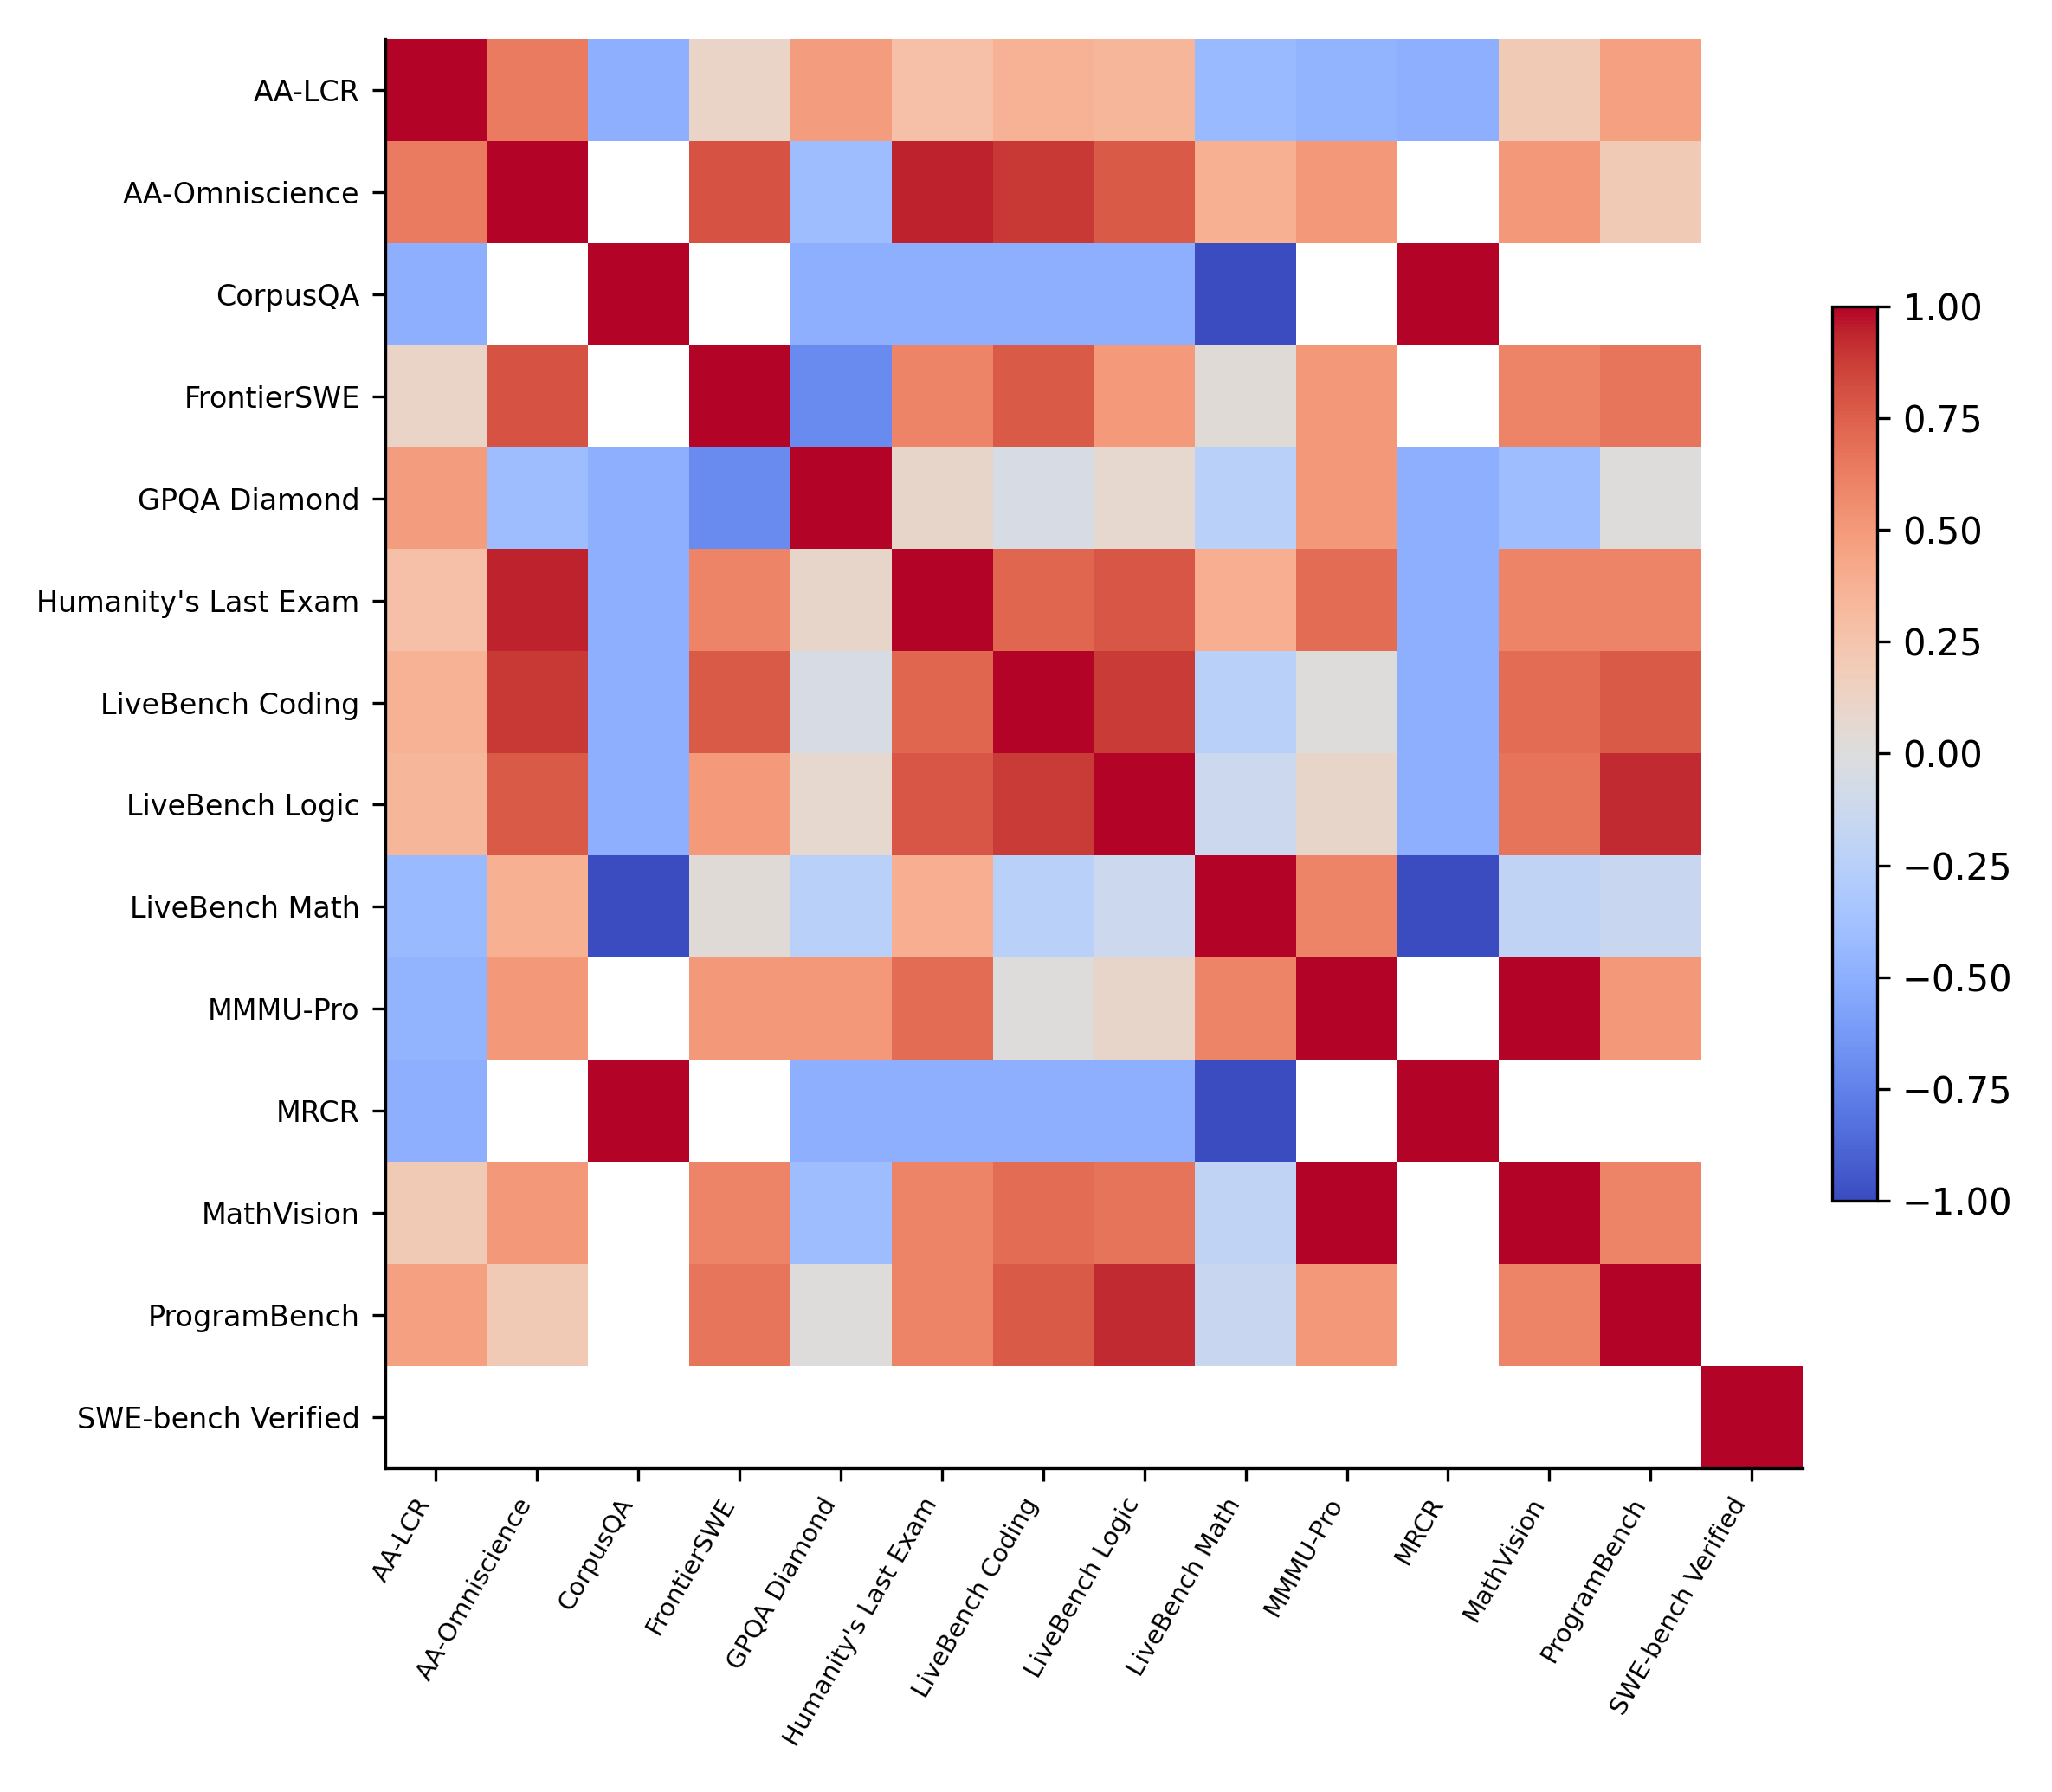
\includegraphics[width=0.86\textwidth]{outputs/q1/figures/figure_q1_02_spearman_heatmap.png}
    \caption{Benchmark Family 缺失感知 Spearman 相关热力图}
    \label{fig:q1_spearman_heatmap}
\end{figure}

本文以 \(|\rho|\geq0.85\) 作为识别高相关候选指标的参考标准，并以 0.80 和 0.90 作为阈值敏感性复核。筛选时不进行机械删除，而综合考虑指标含义、覆盖率、冗余情况和比较网络作用。正式结果见表~\ref{tab:q1_screening}。由表~\ref{tab:q1_screening}可知，虽有 10 个 Benchmark Families 在阈值 0.85 下被标记为高相关候选，但 frozen v1.0 的正式 Family mapping 保持固定，相关性用于报告冗余风险和后续稳健性分析，而非静默删除指标。

\begin{table}[htbp]
\centering
\caption{Benchmark Family 相关性与筛选结果}
\label{tab:q1_screening}
\resizebox{\textwidth}{!}{
\begin{tabular}{llcccl}
\toprule
维度 & Benchmark Family & 覆盖率 & 最大 \(|\rho|\) & 共同样本数 & 保留原因 \\
\midrule
C1 & GPQA Diamond & 1.000 & 0.700 & 5 & 结构桥接，保留 \\
C1 & LiveBench Logic & 1.000 & 0.928 & 6 & 高相关候选，保留并报告冗余 \\
C1 & LiveBench Math & 1.000 & 1.000 & 3 & 高相关候选，保留并报告冗余 \\
C2 & AA-Omniscience & 1.000 & 0.943 & 6 & 结构桥接，保留并报告冗余 \\
C2 & Humanity's Last Exam & 1.000 & 0.943 & 6 & 结构桥接，保留并报告冗余 \\
C3 & AA-LCR & 1.000 & 0.638 & 6 & 结构桥接，保留 \\
C3 & CorpusQA & 1.000 & 1.000 & 3 & 结构桥接，保留并报告冗余 \\
C3 & MRCR & 1.000 & 1.000 & 3 & 结构桥接，保留并报告冗余 \\
C4 & FrontierSWE & 1.000 & 0.800 & 4 & 结构桥接，保留 \\
C4 & LiveBench Coding & 1.000 & 0.886 & 6 & 高相关候选，保留并报告冗余 \\
C4 & ProgramBench & 1.000 & 0.928 & 6 & 结构桥接，保留并报告冗余 \\
C4 & SWE-bench Verified & 1.000 & -- & 0 & 结构桥接，保留 \\
C5 & MMMU-Pro & 1.000 & 1.000 & 3 & 结构桥接，保留并报告冗余 \\
C5 & MathVision & 1.000 & 1.000 & 3 & 结构桥接，保留并报告冗余 \\
\bottomrule
\end{tabular}}
\end{table}

\subsection{成对比较构造}

不同 Benchmark 的评分范围和测试协议存在差异，因此本文只在同一 Exact Setting 内比较模型表现。设模型 \(i\) 与模型 \(j\) 在测试设置 \(s\) 上的成绩分别为 \(x_{is}\) 和 \(x_{js}\)，则定义成对比较结果为
\begin{equation}
y_{ijs}
=
\begin{cases}
1, & x_{is}>x_{js},\\
0.5, & x_{is}=x_{js},\\
0, & x_{is}<x_{js}.
\end{cases}
\label{eq:q1_pair_result}
\end{equation}
当任一模型在该设置上不存在有效成绩时，不构造成对比较关系。

仅使用胜负关系会将微弱领先和显著领先视为等价。为保留性能差距信息，定义模型 \(i\) 与模型 \(j\) 在设置 \(s\) 上的归一化性能差距为
\begin{equation}
m_{ijs}
=
\frac{|x_{is}-x_{js}|}
{\max_l x_{ls}-\min_l x_{ls}+\varepsilon}.
\label{eq:q1_margin}
\end{equation}
进一步定义 Margin 权重
\begin{equation}
w^{(m)}_{ijs}
=
\varepsilon_m+(1-\varepsilon_m)m_{ijs}.
\label{eq:q1_pair_weight_margin}
\end{equation}
为避免包含较多 Exact Settings 的 Benchmark Family 获得更高隐含权重，本文在每个能力维度内部进行 Family balancing。最终单个成对比较权重为
\begin{equation}
w_{ijs}
=
w^{(m)}_{ijs}w^{(f)}_s,
\label{eq:q1_pair_weight}
\end{equation}
其中 \(w^{(f)}_s\) 为经 Exact Setting 和 Benchmark Family 两级归一化后的平衡权重。式~\eqref{eq:q1_margin}--式~\eqref{eq:q1_pair_weight} 保证差距较大的同设置比较提供更强证据，同时避免某一测试体系因设置数量多而被重复计权。

\subsection{Bradley--Terry 模型}

在第 \(d\) 个能力维度上，设模型 \(i\) 的潜在能力参数为 \(\theta_{id}\)。Bradley--Terry 模型给出模型 \(i\) 优于模型 \(j\) 的概率：
\begin{equation}
P(i\succ j)
=
\frac{\exp(\theta_{id})}
{\exp(\theta_{id})+\exp(\theta_{jd})}
=
\sigma(\theta_{id}-\theta_{jd}).
\label{eq:q1_bt}
\end{equation}
根据所有有效成对比较 \(r\)，加权对数似然为
\begin{equation}
\ell_d(\boldsymbol{\theta})
=
\sum_r
w_r
\left[
y_r\ln p_r
+(1-y_r)\ln(1-p_r)
\right].
\label{eq:q1_bt_likelihood}
\end{equation}
部分维度中存在完全分离或近完全分离风险，因此本文加入 \(L_2\) 正则项，估计目标为
\begin{align}
\hat{\boldsymbol{\theta}}_d
&=
\arg\min_{\boldsymbol{\theta}}
\left\{
-\ell_d(\boldsymbol{\theta})
+\frac{\lambda}{2}\sum_i\theta_{id}^{2}
\right\}, \notag\\
\text{s.t.}\quad
&\sum_i\theta_{id}=0.
\label{eq:q1_bt_loss}
\end{align}
式~\eqref{eq:q1_bt_loss} 中 \(\lambda=1.0\) 为主模型正则化参数。为增强潜在能力参数的直观性，将每个维度内的 Bradley--Terry 参数转化至 \(0\sim100\) 区间：
\begin{equation}
S_{id}
=
100
\frac{
\hat{\theta}_{id}-\min_i\hat{\theta}_{id}
}{
\max_i\hat{\theta}_{id}-\min_i\hat{\theta}_{id}
}.
\label{eq:q1_dimension_score}
\end{equation}
式~\eqref{eq:q1_dimension_score} 的标准化仅发生在同一能力维度内部，其作用是提高结果可解释性，并不将不同 Benchmark 的原始分数进行跨尺度直接比较。

各模型五维能力得分见表~\ref{tab:q1_dimension_scores}，对应热力图见图~\ref{fig:q1_dimension_scores}。由表~\ref{tab:q1_dimension_scores} 和图~\ref{fig:q1_dimension_scores}可知，不同模型的能力结构存在明显差异，Kimi K3 在 C4 代码与软件工程和 C3 长上下文上相对突出。

\begin{table}[htbp]
\centering
\caption{各模型五维能力得分}
\label{tab:q1_dimension_scores}
\resizebox{\textwidth}{!}{
\begin{tabular}{lccccc}
\toprule
模型 & C1 & C2 & C3 & C4 & C5 \\
\midrule
Kimi K3 (max reasoning) & 80.222 & 46.257 & 66.362 & 93.780 & 34.569 \\
GPT-5.6 Sol (max) & 80.618 & 59.358 & 54.028 & 73.955 & 100.000 \\
GPT-5.5 (xhigh) & 88.998 & 36.467 & 57.731 & 38.556 & 6.974 \\
Claude Fable 5 (max, with fallback) & 48.008 & 100.000 & 51.063 & 100.000 & 61.411 \\
Claude Opus 4.8 (max) & 100.000 & 45.610 & 40.819 & 45.032 & 0.000 \\
Gemini-3.1-Pro (High) & 95.972 & 41.062 & 0.000 & 52.657 & 59.505 \\
DeepSeek-V4-Pro Max & 37.365 & 0.000 & 100.000 & 93.163 & -- \\
DeepSeek-V4-Flash Max & 0.000 & 16.616 & 49.619 & 0.000 & -- \\
Qwen3.8-Max & 62.030 & 11.369 & 44.436 & 62.073 & 55.082 \\
GLM-5.2 (max) & 29.305 & 9.804 & 51.063 & 24.138 & -- \\
\bottomrule
\end{tabular}}
\end{table}

\begin{figure}[htbp]
    \centering
    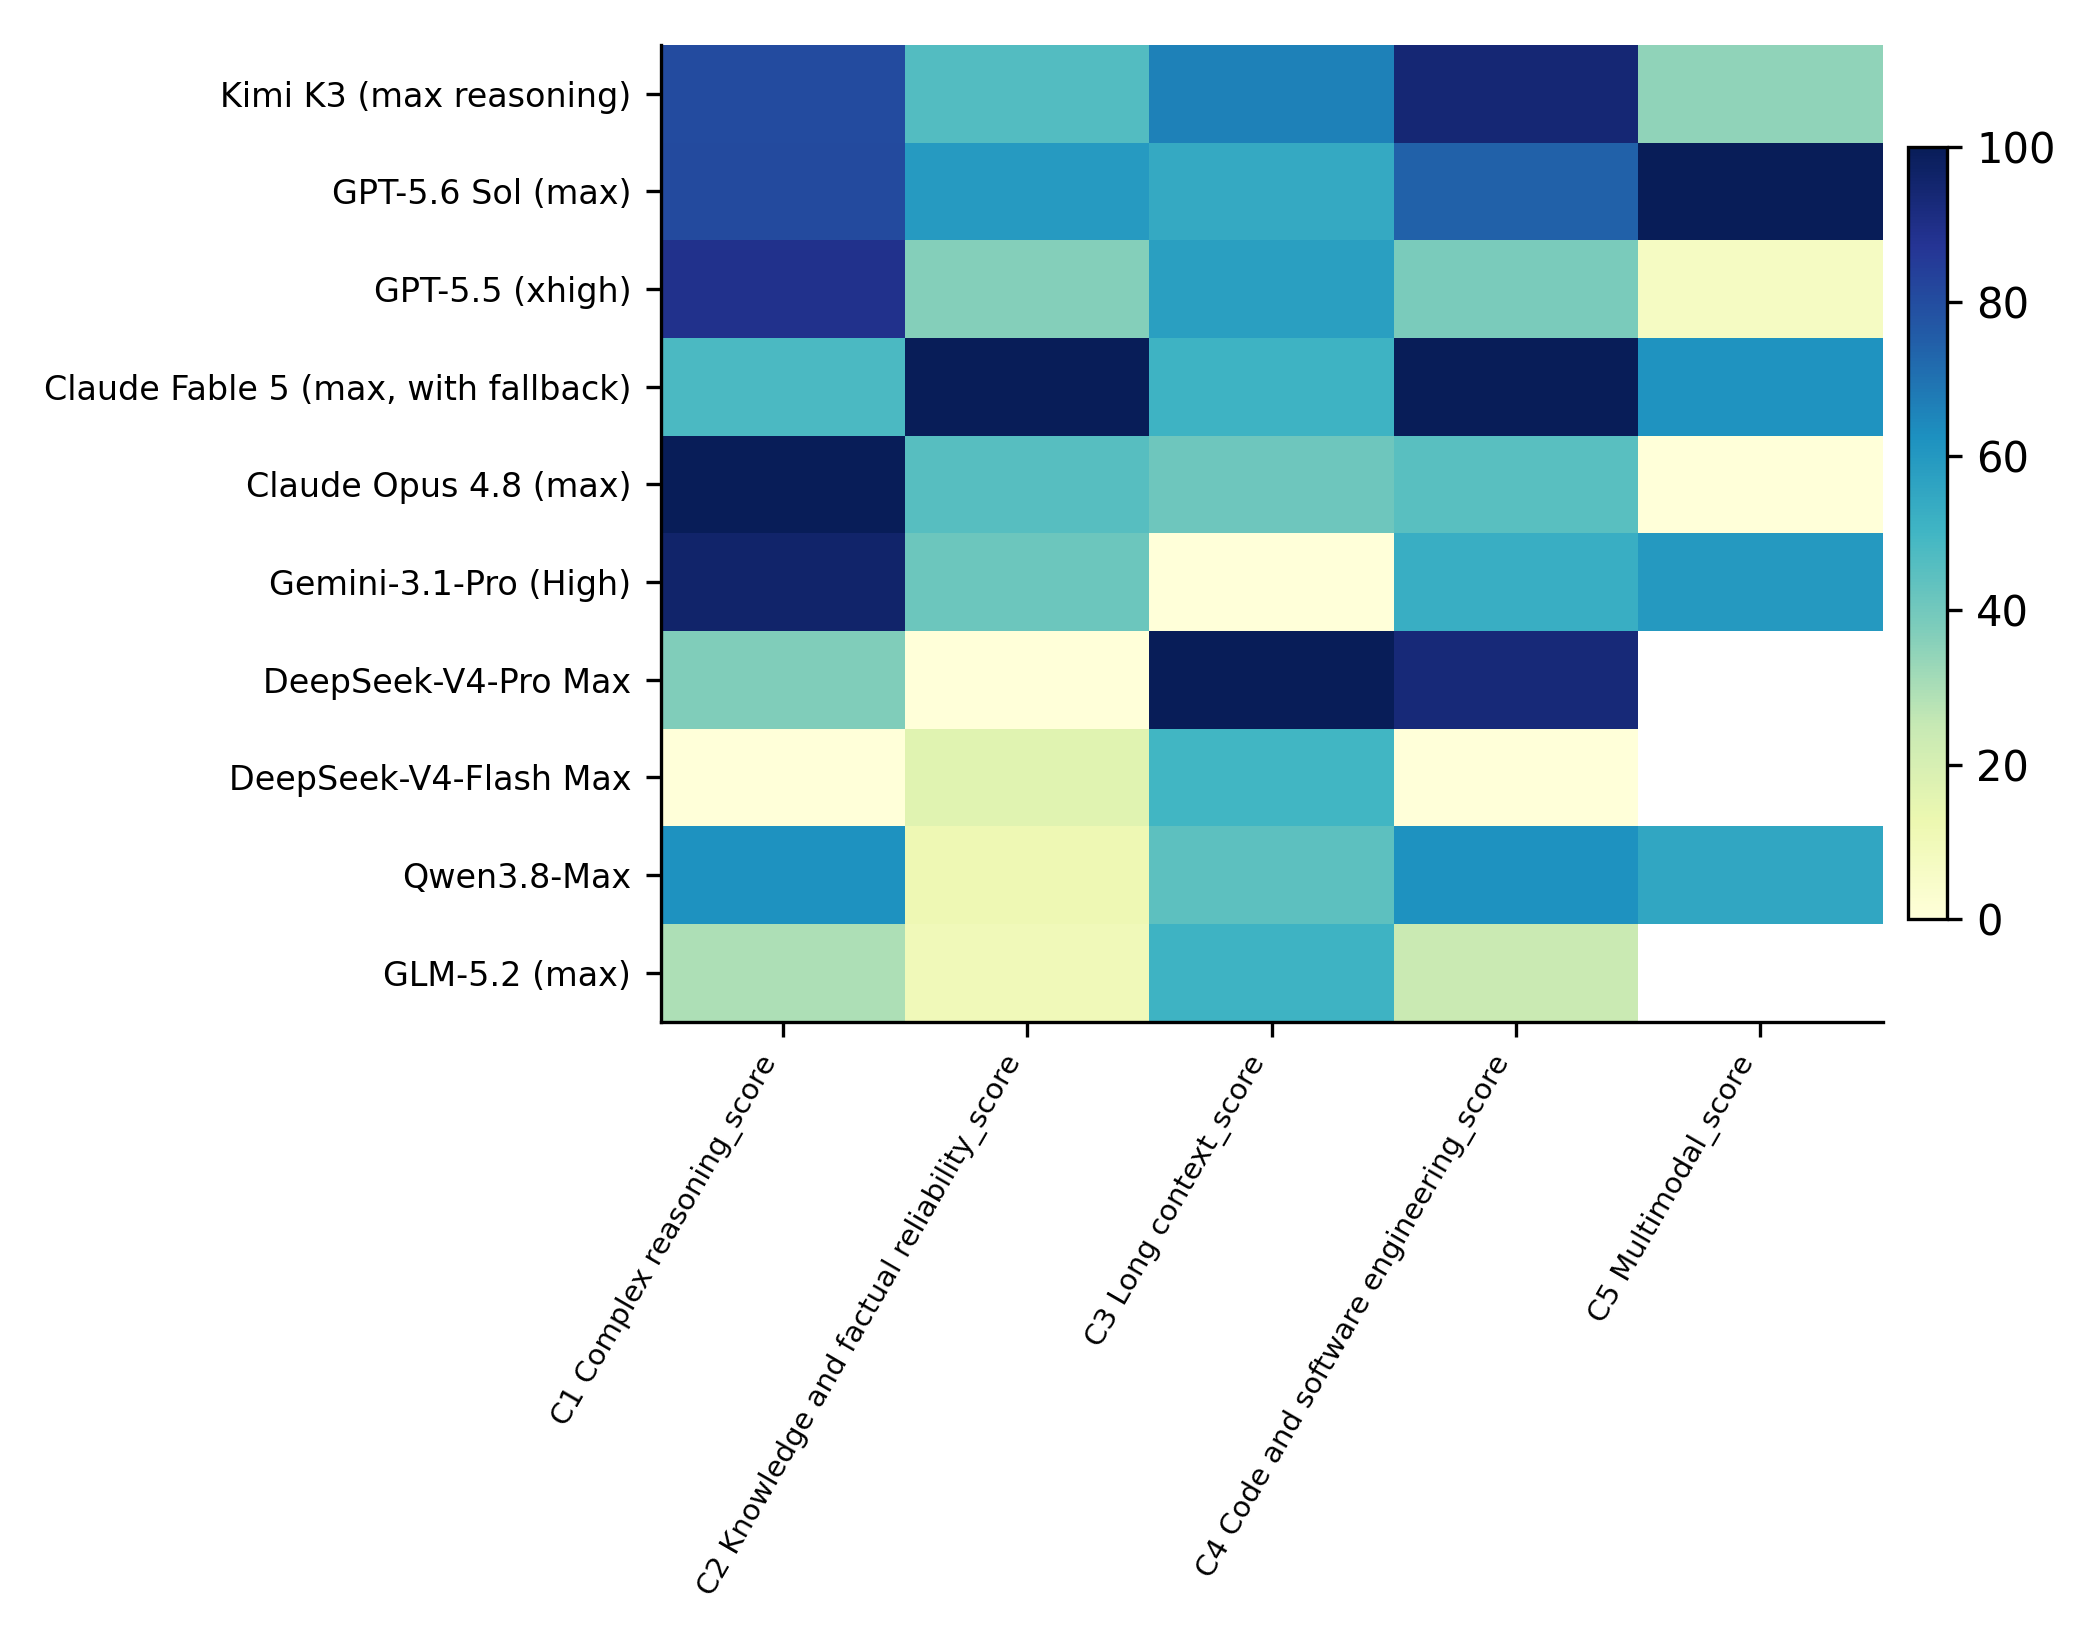
\includegraphics[width=0.78\textwidth]{outputs/q1/figures/figure_q1_04_dimension_scores.png}
    \caption{各模型五维能力得分热力图}
    \label{fig:q1_dimension_scores}
\end{figure}

比较网络诊断表明，C1 比较网络整体较为稳定；C2 存在 separation warning，但正则化 Bradley--Terry 模型能够收敛；C3 在完整数据下连通，但对 AA-LCR 存在结构依赖；C4 对 LiveBench Coding 存在桥接依赖；C5 仅有 7 个模型适用。现有公开评测数据在部分能力维度上的模型比较网络存在局部脆弱性，因此本文进一步通过 LOFO 分析检验单一 Benchmark Family 对结果的影响，并对相关维度中的小幅名次差异作谨慎解释。

\subsection{五维客观权重}

Bradley--Terry 模型得到的是模型在五个能力维度上的相对表现，而五个维度在当前公开评测数据中的有效信息贡献并不相同。因此，本文从信息量、非冗余度和稳定度三个方面确定客观权重。这里的权重表示各维度在当前评价数据集中的有效信息贡献，而不是人为认定各能力本身的重要程度。

令第 \(d\) 个能力维度中模型 \(i\) 的标准化得分为 \(S_{id}\)，定义
\begin{equation}
p_{id}
=
\frac{S_{id}+\varepsilon}
{\sum_i(S_{id}+\varepsilon)}.
\label{eq:q1_information_p}
\end{equation}
归一化信息熵和信息量分别为
\begin{equation}
H_d
=
-\frac{1}{\ln n_d}
\sum_i p_{id}\ln p_{id},
\qquad
I_d=1-H_d.
\label{eq:q1_information}
\end{equation}
若某一维度能够明显区分不同模型，则 \(I_d\) 较高。

在五维能力得分之间重新计算缺失感知 Spearman 系数，定义非冗余度为
\begin{equation}
R_d
=
1-
\frac{1}{D_d}
\sum_{k\neq d}
|\rho_{dk}|,
\label{eq:q1_redundancy}
\end{equation}
其中 \(D_d\) 为与维度 \(d\) 存在有效共同样本的其他维度数量。通过 Bootstrap 重采样得到模型在各维度得分的波动程度，设模型 \(i\) 在第 \(d\) 个维度上的 Bootstrap 标准差为 \(\sigma_{id}^{(B)}\)，定义
\begin{equation}
U_d
=
\operatorname{median}_i
\left(
\sigma_{id}^{(B)}
\right),
\qquad
T_d
=
\frac{1}{1+\widetilde U_d}.
\label{eq:q1_stability}
\end{equation}
最终，第 \(d\) 个能力维度的综合信息贡献和客观权重为
\begin{equation}
q_d=I_dR_dT_d,
\qquad
w_d
=
\frac{q_d}{\sum_{k=1}^{5}q_k}.
\label{eq:q1_dimension_weight}
\end{equation}

五维客观权重结果见表~\ref{tab:q1_weights}。计算得到
\[
(w_1,w_2,w_3,w_4,w_5)
=
(0.0134,\ 0.3399,\ 0.1997,\ 0.0600,\ 0.3870).
\]
由表~\ref{tab:q1_weights}可知，C5 和 C2 在当前数据条件下具有较高的信息贡献，C1 的客观权重较低。这一结果意味着 C1 在当前 10 个模型和现有公开评测数据上提供的新增区分信息相对有限，不能解释为复杂推理能力本身不重要。

\begin{table}[htbp]
\centering
\caption{五维能力客观权重及其构成}
\label{tab:q1_weights}
\begin{tabular}{lcccc}
\toprule
维度 & 信息量 \(I_d\) & 非冗余度 \(R_d\) & 稳定度 \(T_d\) & 权重 \(w_d\) \\
\midrule
C1 复杂推理 & 0.0754 & 0.6581 & 0.0669 & 0.0134 \\
C2 知识与事实可靠性 & 0.1360 & 0.6189 & 1.0000 & 0.3399 \\
C3 长上下文 & 0.0620 & 0.7981 & 1.0000 & 0.1997 \\
C4 代码与软件工程 & 0.0812 & 0.5950 & 0.3076 & 0.0600 \\
C5 多模态 & 0.1651 & 0.5804 & 1.0000 & 0.3870 \\
\bottomrule
\end{tabular}
\end{table}

\subsection{综合评价}

对于模型 \(i\)，设其具有有效评价结果的能力维度集合为 \(D_i\)。考虑到不同模型的数据适用范围并不完全相同，本文采用有效权重重新归一化的方法计算综合得分：
\begin{equation}
G_i
=
\frac{
\sum_{d\in D_i}w_dS_{id}
}{
\sum_{d\in D_i}w_d
}.
\label{eq:q1_overall_score}
\end{equation}
同时定义有效权重覆盖率为
\begin{equation}
C_i
=
\sum_{d\in D_i}w_d.
\label{eq:q1_effective_coverage}
\end{equation}
式~\eqref{eq:q1_overall_score} 和式~\eqref{eq:q1_effective_coverage} 避免了将未公开或不适用维度直接赋值为零，同时将模型综合评分所使用的信息完整程度显式呈现。特别地，C5 缺失模型的多模态得分在表中记为“--”，不参与该模型综合得分分子和分母的计算。

综合得分和排名见表~\ref{tab:q1_overall_ranking}，综合得分及 Bootstrap 置信区间见图~\ref{fig:q1_overall_ci}。由表~\ref{tab:q1_overall_ranking}可知，GPT-5.6 Sol (max)、Claude Fable 5 (max, with fallback) 和 Kimi K3 (max reasoning) 分别位列前三，得分为 75.183、74.599 和 49.056。由图~\ref{fig:q1_overall_ci}可知，前两名位于第一梯队，Kimi K3 与其后的 DeepSeek-V4-Pro Max、Gemini-3.1-Pro (High) 等模型存在一定得分差距。

\begin{table}[htbp]
\centering
\caption{十款大语言模型综合得分与排名}
\label{tab:q1_overall_ranking}
\resizebox{\textwidth}{!}{
\begin{tabular}{clccccccc}
\toprule
排名 & 模型 & C1 & C2 & C3 & C4 & C5 & 综合得分 & 有效权重覆盖率 \\
\midrule
1 & GPT-5.6 Sol (max) & 80.618 & 59.358 & 54.028 & 73.955 & 100.000 & 75.183 & 1.000 \\
2 & Claude Fable 5 (max, with fallback) & 48.008 & 100.000 & 51.063 & 100.000 & 61.411 & 74.599 & 1.000 \\
3 & Kimi K3 (max reasoning) & 80.222 & 46.257 & 66.362 & 93.780 & 34.569 & 49.056 & 1.000 \\
4 & DeepSeek-V4-Pro Max & 37.365 & 0.000 & 100.000 & 93.163 & -- & 42.509 & 0.613 \\
5 & Gemini-3.1-Pro (High) & 95.972 & 41.062 & 0.000 & 52.657 & 59.505 & 41.433 & 1.000 \\
6 & Qwen3.8-Max & 62.030 & 11.369 & 44.436 & 62.073 & 55.082 & 38.610 & 1.000 \\
7 & GPT-5.5 (xhigh) & 88.998 & 36.467 & 57.731 & 38.556 & 6.974 & 30.129 & 1.000 \\
8 & Claude Opus 4.8 (max) & 100.000 & 45.610 & 40.819 & 45.032 & 0.000 & 27.698 & 1.000 \\
9 & DeepSeek-V4-Flash Max & 0.000 & 16.616 & 49.619 & 0.000 & -- & 25.374 & 0.613 \\
10 & GLM-5.2 (max) & 29.305 & 9.804 & 51.063 & 24.138 & -- & 25.071 & 0.613 \\
\bottomrule
\end{tabular}}
\end{table}

\begin{figure}[htbp]
    \centering
    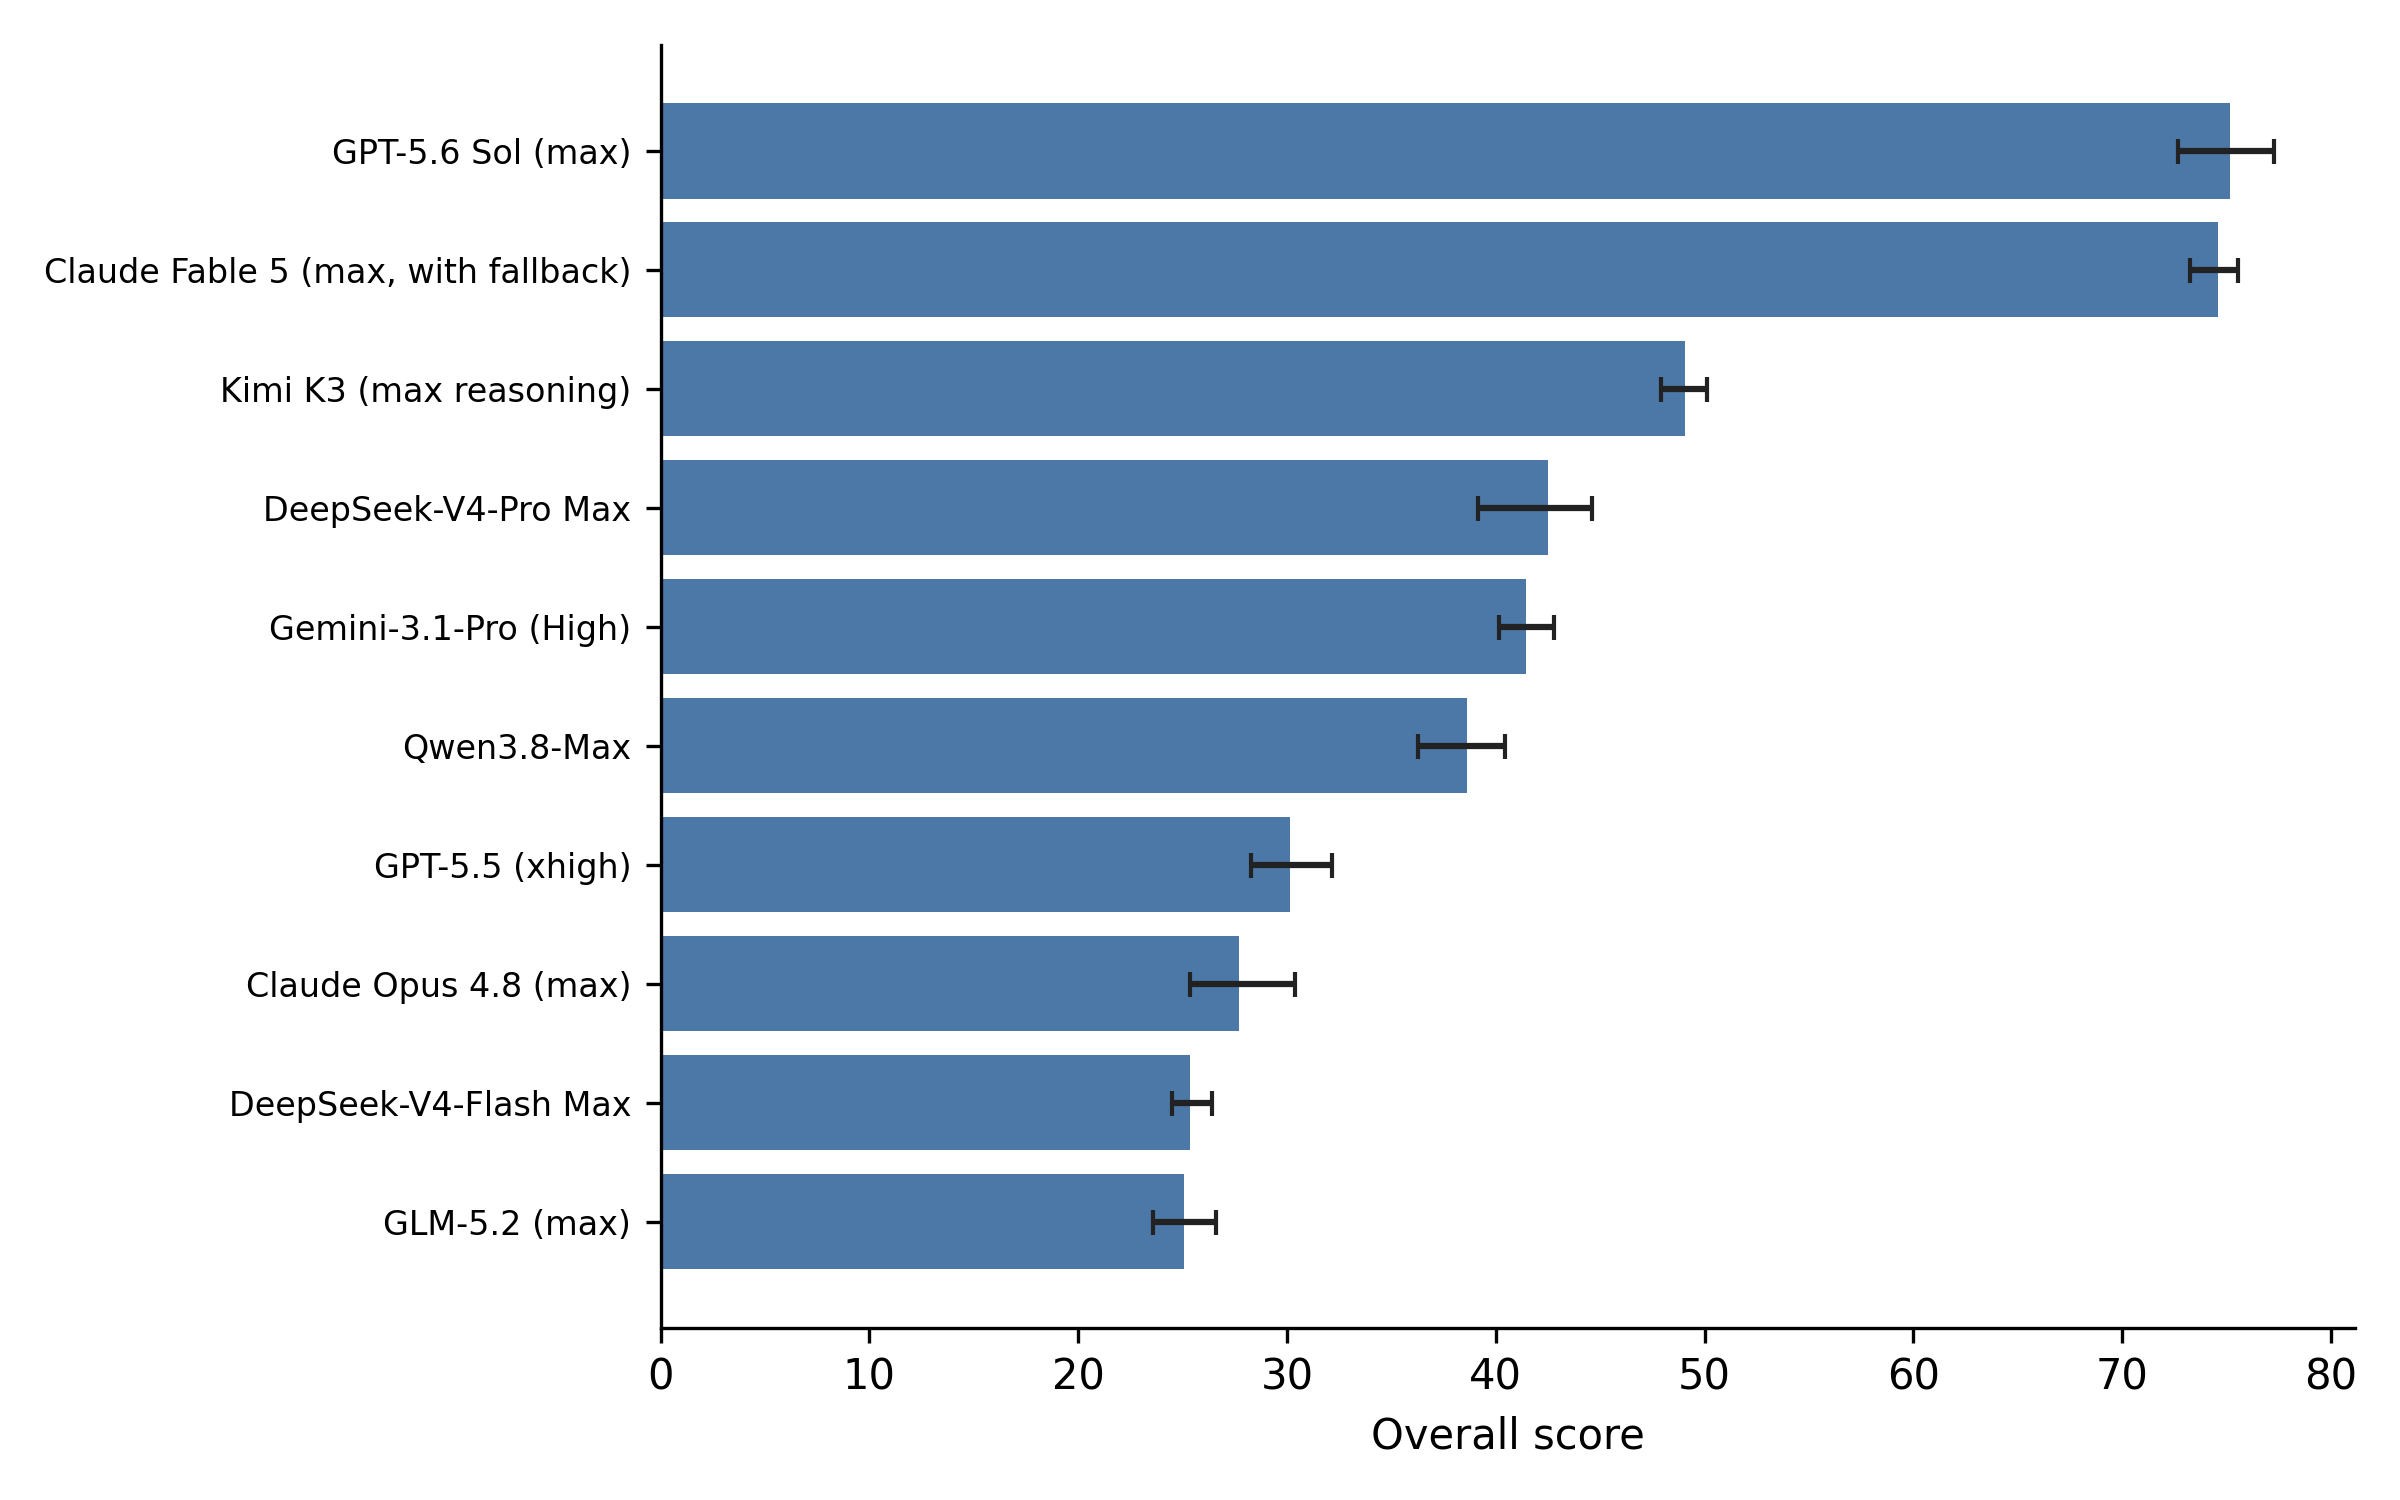
\includegraphics[width=0.82\textwidth]{outputs/q1/figures/figure_q1_05_overall_score_ci.png}
    \caption{综合得分及 95\% Bootstrap 置信区间}
    \label{fig:q1_overall_ci}
\end{figure}

\subsection{稳健性分析}

\subsubsection{Bootstrap 稳定性检验}

为考察有限 Benchmark 样本对结果的影响，本文采用保持 Benchmark Family 层次结构的 Bootstrap 重采样方法，对整个评价流程重复计算 \(B=2000\) 次。每次重采样均重新完成成对比较构建、Bradley--Terry 能力估计、五维客观赋权和综合评分。

对于模型 \(i\)，定义其进入前三名的概率为
\begin{equation}
P_i^{\mathrm{Top3}}
=
\frac{1}{B}
\sum_{b=1}^{B}
\mathbf{1}\!\left(r_i^{(b)}\leq3\right).
\label{eq:q1_top3}
\end{equation}
Bootstrap 排名稳定性见图~\ref{fig:q1_rank_stability}。由图~\ref{fig:q1_rank_stability}可知，Kimi K3 的 Bootstrap 排名区间为第 3 名到第 3 名，进入前三名的概率为 1.000，说明其在本题样本中的综合竞争位置较为稳定。

\begin{figure}[htbp]
    \centering
    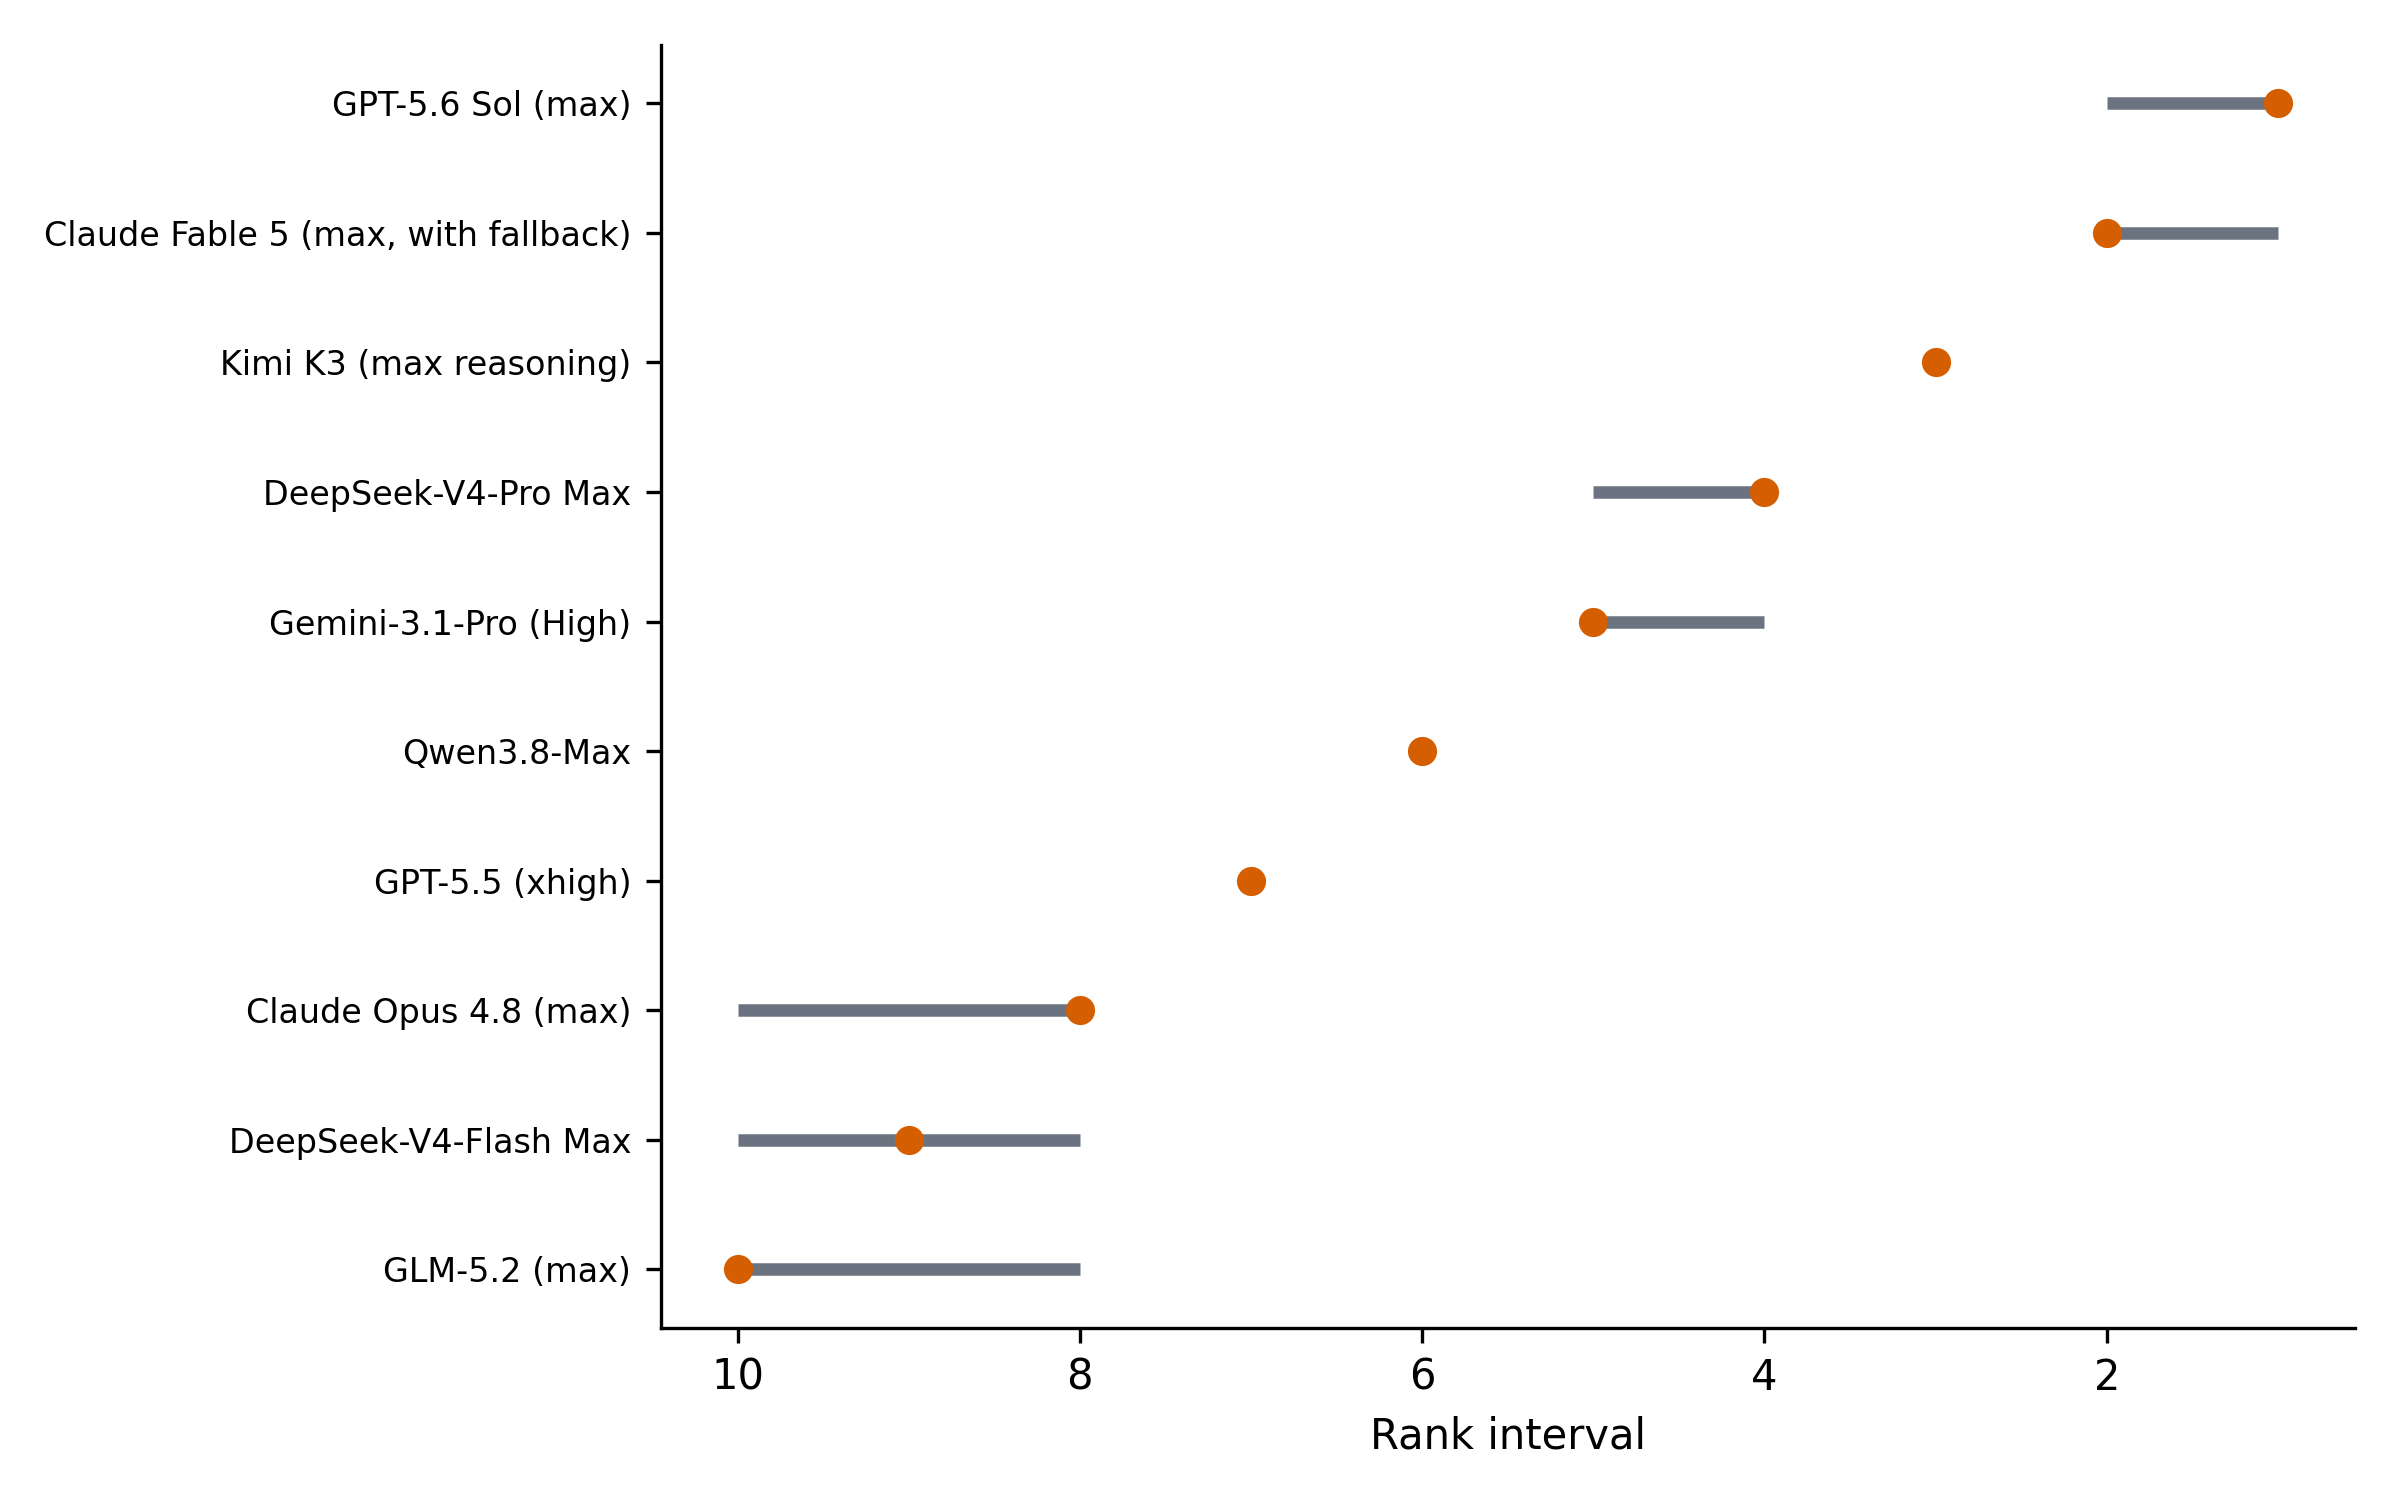
\includegraphics[width=0.82\textwidth]{outputs/q1/figures/figure_q1_06_rank_stability.png}
    \caption{Bootstrap 排名稳定性}
    \label{fig:q1_rank_stability}
\end{figure}

\subsubsection{LOFO 与模型设定敏感性}

为检验单一 Benchmark Family 对结果的影响，本文依次删除 14 个 Benchmark Families 中的一个，并重新运行完整评价模型。对模型 \(i\) 和被删除的 Benchmark Family \(f\)，定义排名变化为
\begin{equation}
\Delta r_{if}
=
r_{i,-f}-r_i,
\label{eq:q1_lofo}
\end{equation}
其中 \(r_i\) 为完整模型下排名，\(r_{i,-f}\) 为删除 \(f\) 后的排名。

LOFO 排名变化见图~\ref{fig:q1_lofo}。由图~\ref{fig:q1_lofo}可知，大多数单一 Benchmark Family 的删除不会彻底改变总体竞争格局，但部分来源会影响相邻模型次序。结合网络诊断结果，C3 对 AA-LCR 有结构依赖，C4 对 LiveBench Coding 有桥接依赖。该现象说明当前公开评测数据在长上下文和代码能力维度仍存在一定测评来源集中性，对这些维度中的小幅分数差异不宜作过度解释。

\begin{figure}[htbp]
    \centering
    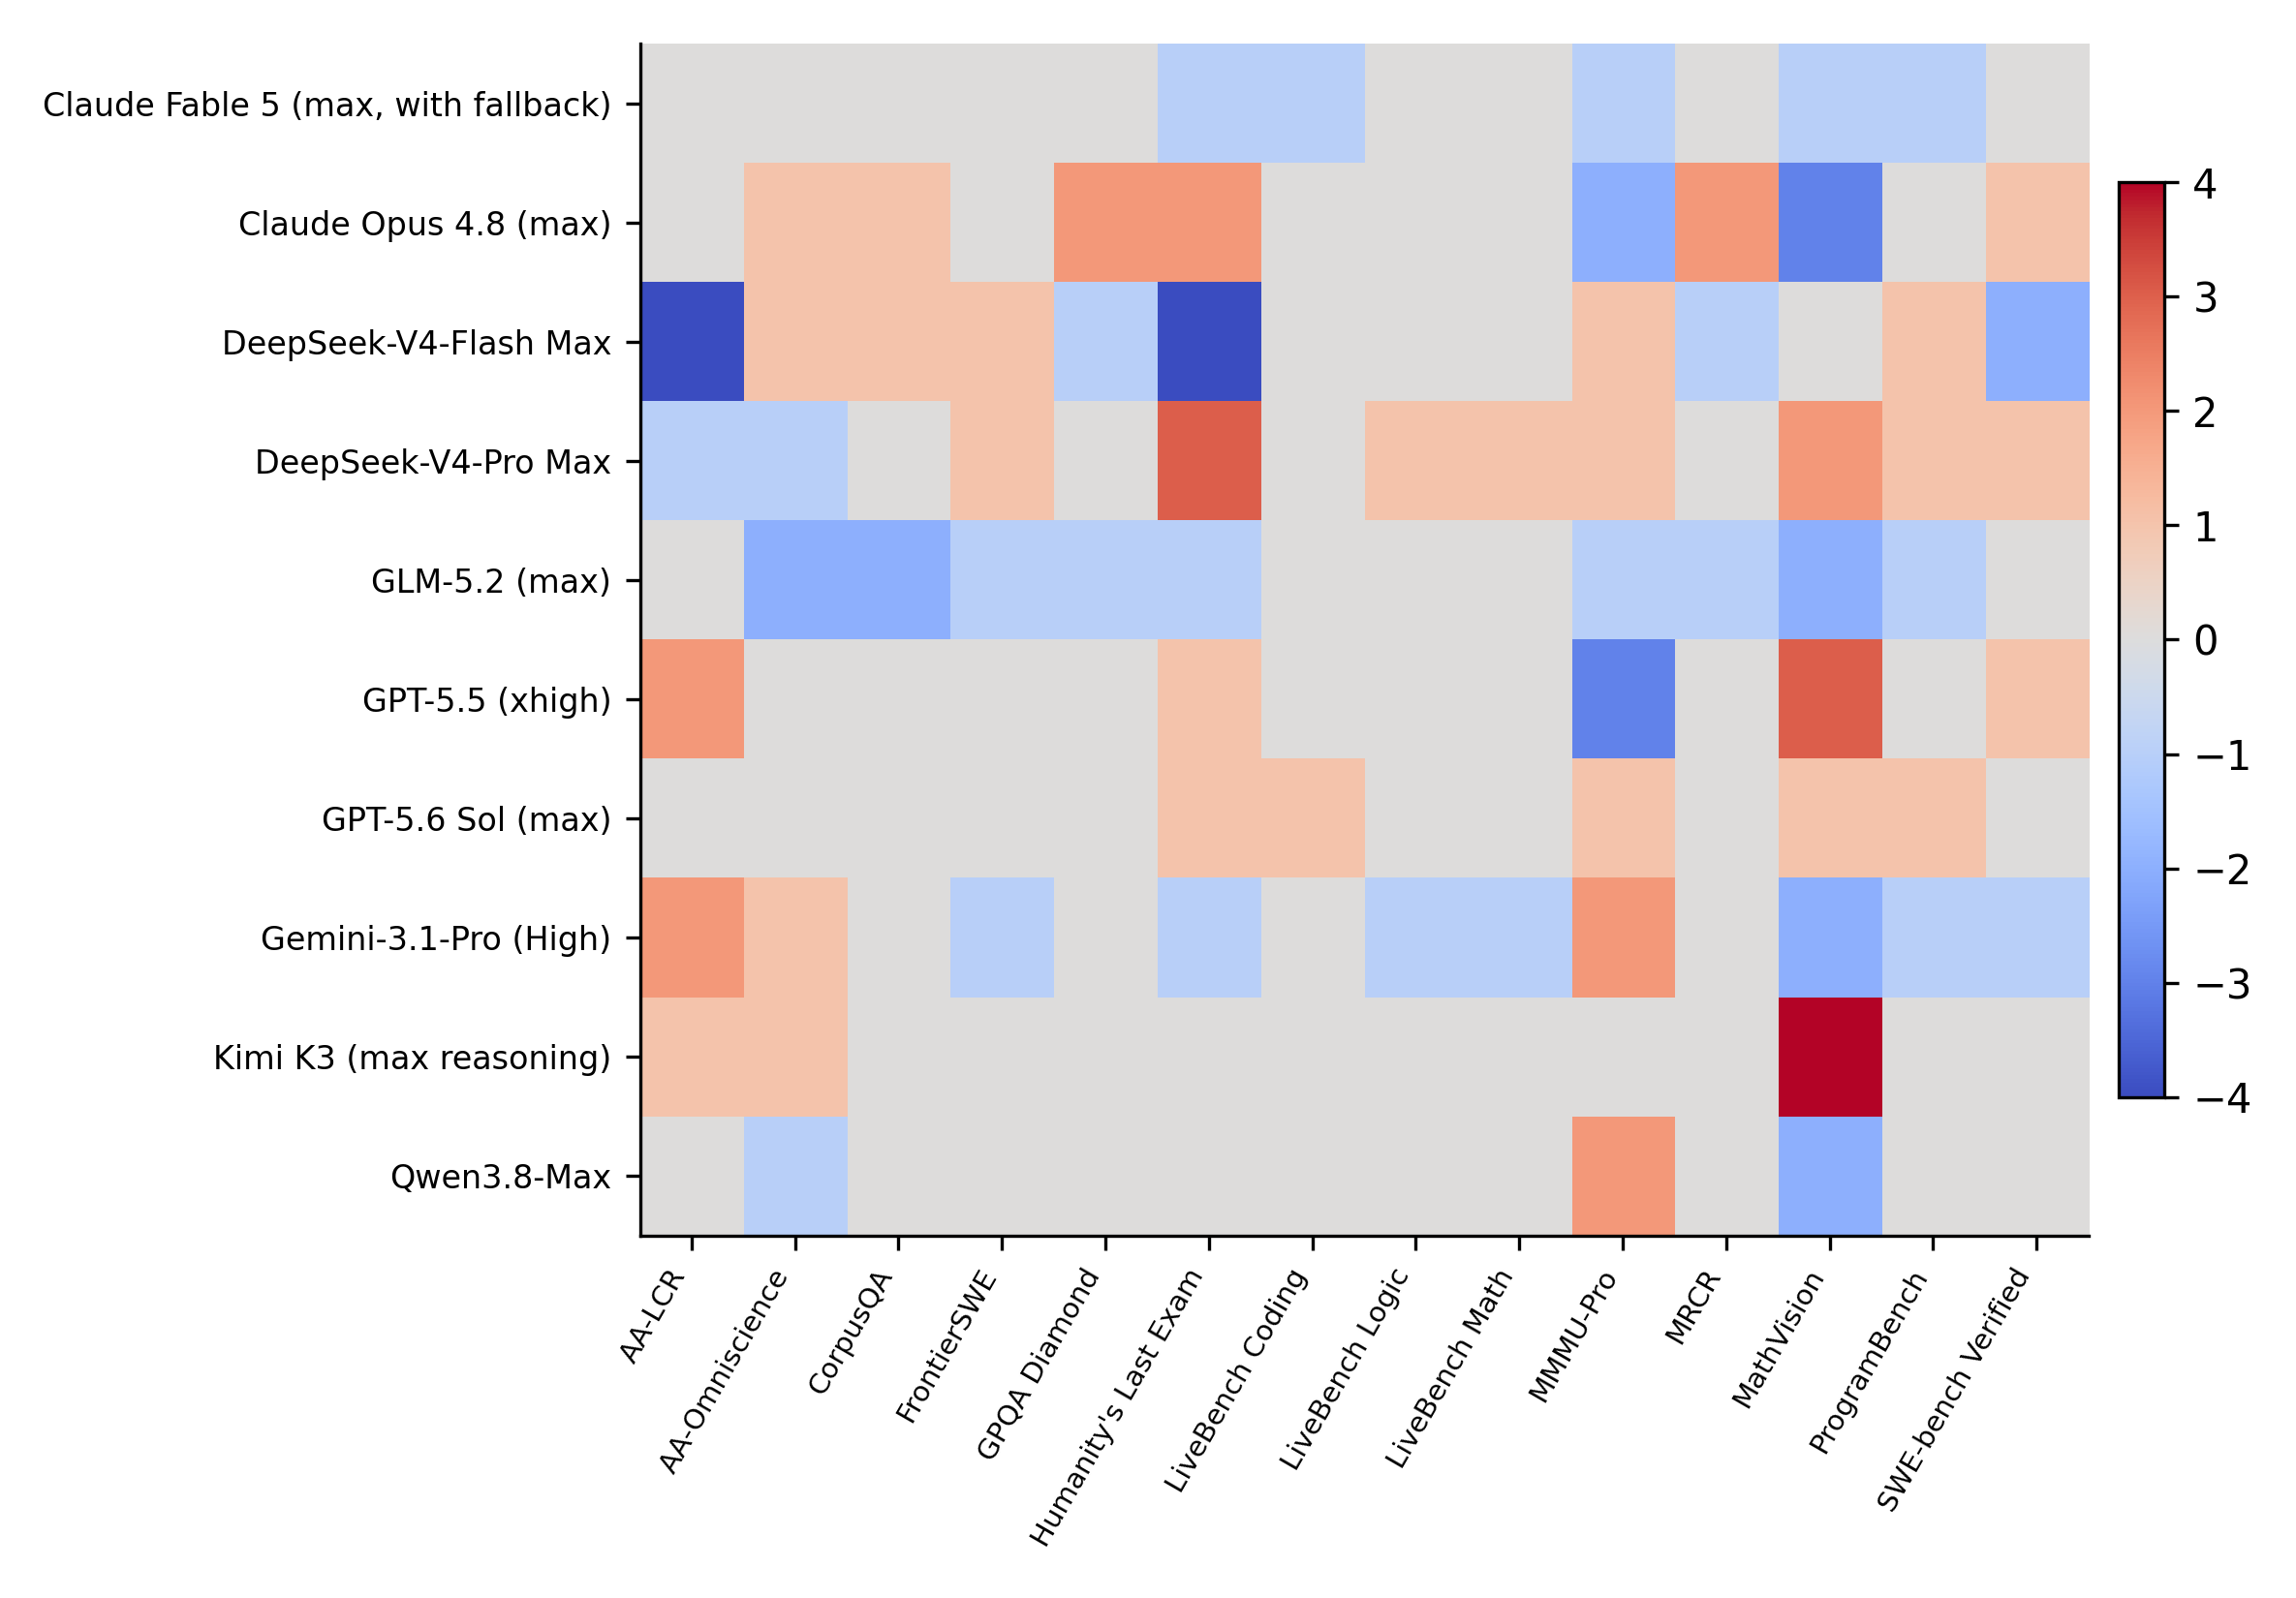
\includegraphics[width=0.86\textwidth]{outputs/q1/figures/figure_q1_07_lofo_rank_change.png}
    \caption{Leave-One-Family-Out 排名变化}
    \label{fig:q1_lofo}
\end{figure}

除 LOFO 外，本文进一步改变正则化参数、Margin weighting 方法，并考察删除 C5、多模态完整样本子集和五维等权等情景。关键稳健性结果见表~\ref{tab:q1_kimi_robustness}。由表~\ref{tab:q1_kimi_robustness}可知，删除 C5 对总体排名结构影响较大，Spearman 秩相关降至 0.794，但 Kimi K3 的排名未改变；删除 AA-LCR 或取消 Margin weighting 时，Kimi K3 排名下降 1 位。

\begin{table}[htbp]
\centering
\caption{Kimi K3 的 Bootstrap 和敏感性结果}
\label{tab:q1_kimi_robustness}
\begin{tabular}{lccc}
\toprule
检验项 & 关键指标 & 数值 & Kimi 排名变化 \\
\midrule
主模型 & 综合得分 & 49.056 & 0 \\
Bootstrap & Top-3 概率 & 1.000 & 0 \\
Bootstrap & 95\% 得分区间 & [47.911, 50.096] & 0 \\
删除 C5 & Spearman / Kendall & 0.794 / 0.644 & 0 \\
删除 AA-LCR & Spearman / Kendall & 0.842 / 0.689 & +1 \\
取消 Margin weighting & Spearman / Kendall & 0.879 / 0.733 & +1 \\
五维完整模型子集 & Spearman / Kendall & 1.000 / 1.000 & 0 \\
\bottomrule
\end{tabular}
\end{table}

\subsection{Kimi K3 优劣势分析}

为刻画 Kimi K3 相对于样本模型的能力结构，定义其在维度 \(d\) 上相对于有效模型中位数的差值为
\begin{equation}
A_d
=
S_{\mathrm{Kimi},d}
-
\operatorname{median}_{i\in\mathcal{M}_d}(S_{id}),
\label{eq:q1_kimi_gap}
\end{equation}
其中 \(\mathcal{M}_d\) 为维度 \(d\) 上具有有效得分的模型集合。若 \(A_d>0\)，表示 Kimi K3 在该维度高于有效模型中位水平；反之则表示该维度存在相对短板。

Kimi K3 相对于模型中位数的能力差值见图~\ref{fig:q1_kimi_gap}。由图~\ref{fig:q1_kimi_gap}可知，Kimi K3 最强相对维度为 C4 代码与软件工程，较有效模型中位数高出 36.415 分；最弱相对维度为 C5 多模态，较有效模型中位数低 20.513 分。

\begin{figure}[htbp]
    \centering
    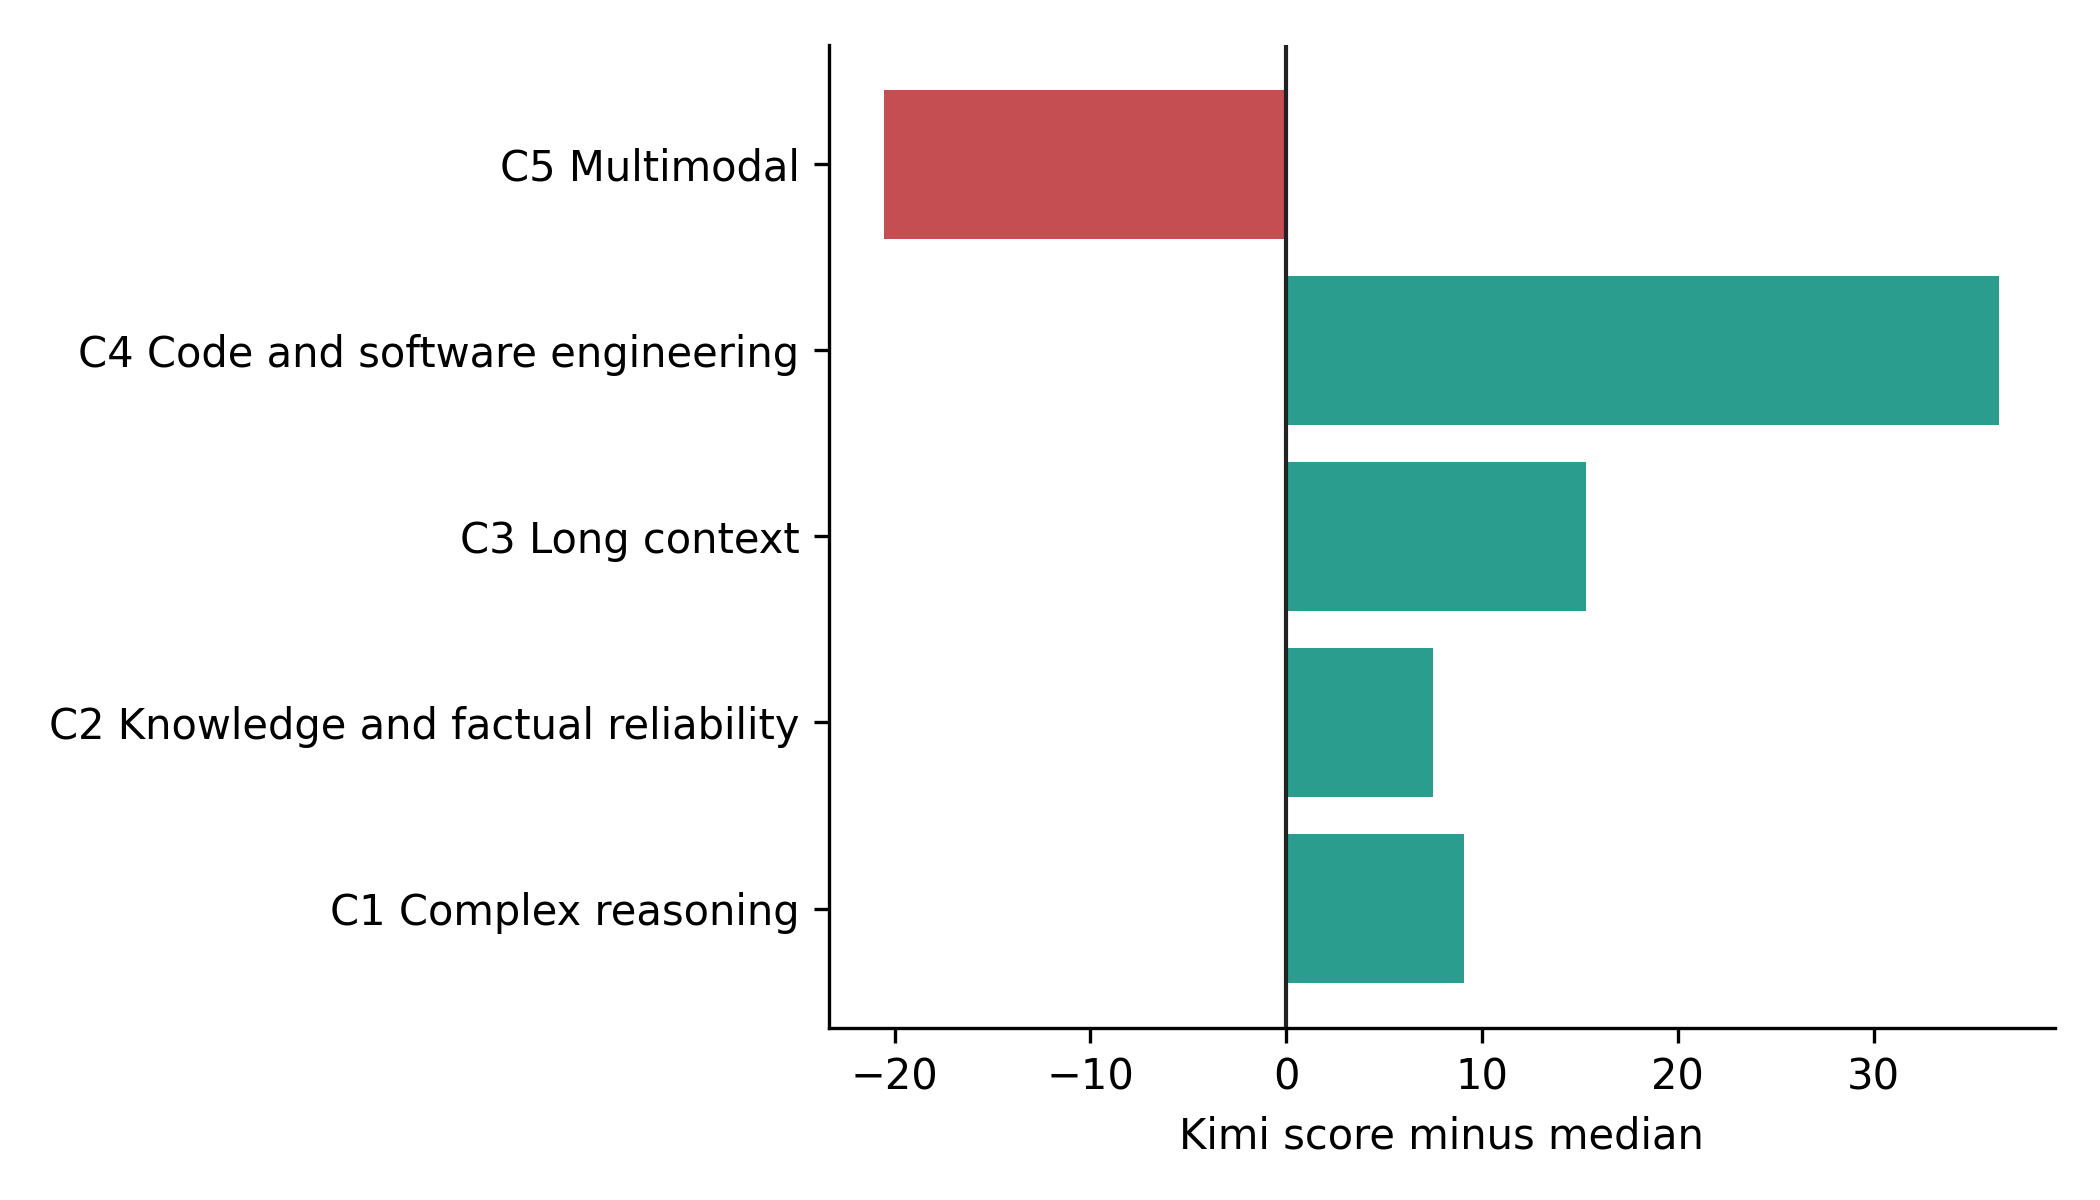
\includegraphics[width=0.68\textwidth]{outputs/q1/figures/figure_q1_10_kimi_advantage_gap.png}
    \caption{Kimi K3 相对于有效模型中位数的能力差值}
    \label{fig:q1_kimi_gap}
\end{figure}

综合来看，Kimi K3 的能力结构具有较鲜明的特点：其代码与软件工程能力表现突出，长上下文能力也高于样本中位水平；多模态能力是当前相对明显的短板。最终综合评价中，Kimi K3 得分为 49.056，排名第 3，Bootstrap 进入前三概率为 1.000，说明其在本文样本模型、现有公开 Benchmark 和当前数据版本下呈现出较稳定的综合竞争优势。但敏感性分析同时表明，删除 AA-LCR 或取消性能差距加权后，其名次均下降 1 位，因此对相邻模型之间的细微名次差异仍需结合指标结构谨慎解释。

\subsection{本问小结}

针对主流大语言模型公开评测指标尺度不统一、同类指标存在信息冗余以及数据不完全等特点，本文建立了基于成对比较的大语言模型综合性能评价方法。首先，利用缺失感知 Spearman 相关系数分析 Benchmark Families 之间的信息重叠关系，并结合数据覆盖程度和模型比较网络连通性完成指标筛选；其次，仅在相同 Exact Setting 内构造模型胜负关系，并进一步考虑性能差距和 Benchmark Family 平衡，建立正则化 Bradley--Terry 模型，获得模型在 C1--C5 五个能力维度上的相对能力得分；随后，从信息量、非冗余度与 Bootstrap 稳定性三个方面确定能力维度的客观信息权重，并通过缺失感知的权重重新归一化得到模型综合得分。

计算结果表明，GPT-5.6 Sol (max)、Claude Fable 5 (max, with fallback) 和 Kimi K3 (max reasoning) 分别位居综合评价前三位，其中 Kimi K3 综合得分为 49.056，在 2000 次 Bootstrap 中进入前三名的概率为 1.000。能力分解进一步表明，Kimi K3 的主要优势集中于 C4 代码与软件工程维度，相对有效模型中位数为 \(+36.415\)；主要短板为 C5 多模态维度，相对有效模型中位数为 \(-20.513\)。此外，LOFO 及多种敏感性检验表明，整体竞争格局具有一定稳定性，但 C3 对 AA-LCR、C4 对 LiveBench Coding 存在结构依赖，且 C5 的有效模型覆盖范围相对有限。因此，本文结论仅针对本题选取模型、现有公开 Benchmark 和当前 frozen v1.0 数据版本成立，对局部维度和相邻名次差异应作谨慎解释。
